
% Slideshow, written by Brent Baccala, for a lecture at Catholic University

\documentclass{beamer}
\usetheme{Madrid}

\title{Alternate techniques for solving systems of polynomial equations}
\author{Brent Baccala}
\institute{\tt cosine@freesoft.org}
\date{February 8, 2023}

\setbeamertemplate{footline}{}
\beamertemplatenavigationsymbolsempty

\usepackage{xcolor}
\usepackage{comment}
\usepackage{graphicx}

\usepackage{tabularx}

\begin{document}


\begin{frame}
\titlepage
\begin{block}{Abstract}
\tiny
While Buchberger's algorithm to construct Gr\"obner bases has justifiably been the subject of study and acclaim since its introduction in 1965, alternate strategies and algorithms exist to solve systems of polynomial equations.  Numerical techniques can be used to construct witness points, which are approximate solutions accurate enough that exact solutions can be recovered from them.  This talk will outline a basic technique for recovering exact solutions from witness points and describe two numerical algorithms used to construct witness points: the homotopy continuation method used by the Bertini software program, and the root finding algorithm used by the speaker to study differential equations.
\end{block}
\end{frame}

\begin{frame}
\begin{exampleblock}{}
\begin{center}
\vskip 20pt
\Huge
Part 1: Gr\"obner and Bertini
\vskip 6pt
\ 
\end{center}
\end{exampleblock}
\end{frame}

\begin{frame}
\frametitle{Part 1}
\begin{itemize}
\item START A RECORDER
\item give a simple example of reducing a polynomial mod an ideal using FLINT routine
\item is this a good idea?
\item illustrate the problem; it can be solved using Grobner bases
\item need to specify a monomial ordering: it matters in the multivariate case

\item solving systems of polynomial equations
\item two examples from Prof. Levin's talk: Lagrange multipliers and graph coloring
\item one is always a special case: linear algebra, matrix methods, LU decomposition
\item higher degree polynomials - Gr\"obner bases
\item demonstrate using two examples

\item performance problems with Buchberger's algorithm: the F4 and F5 algorithms
\begin{itemize}
   \item computing a Gr\"obner basis is NP-hard in general
   \item Faug\'ere's F5 algorithm
\end{itemize}
\end{itemize}
\end{frame}

\begin{frame}
\frametitle{Systems of linear polynomials (1 is always a special case)}
\includegraphics[clip, trim=0in 5.4in 0in 0.5in, width=\textwidth, page=13]{LU decomposition - Wikipedia.pdf}
{\tiny Source: Wikipedia}
%%{\tiny Source: @MathType on Twitter}
%%\includegraphics[clip, trim=0in 2.7in 0in 0in, width=\textwidth]{LU.jpeg}

\[
L = \begin{bmatrix} 
    l_{11} & 0 & \dots & 0 \\
    l_{21} & l_{22} & \ddots & 0 \\
    \vdots & \ddots & \ddots & 0 \\
    l_{K1} & \dots  & \dots & l_{KK} 
    \end{bmatrix}
\qquad
U = \begin{bmatrix} 
    u_{11} & u_{12} & \dots  & u_{1K}\\
         0 & u_{22} & \ddots & \vdots\\
    \vdots & \ddots & \ddots & \vdots\\
         0 & \dots  &    0   & u_{KK} 
    \end{bmatrix}
\]
\end{frame}

\begin{frame}
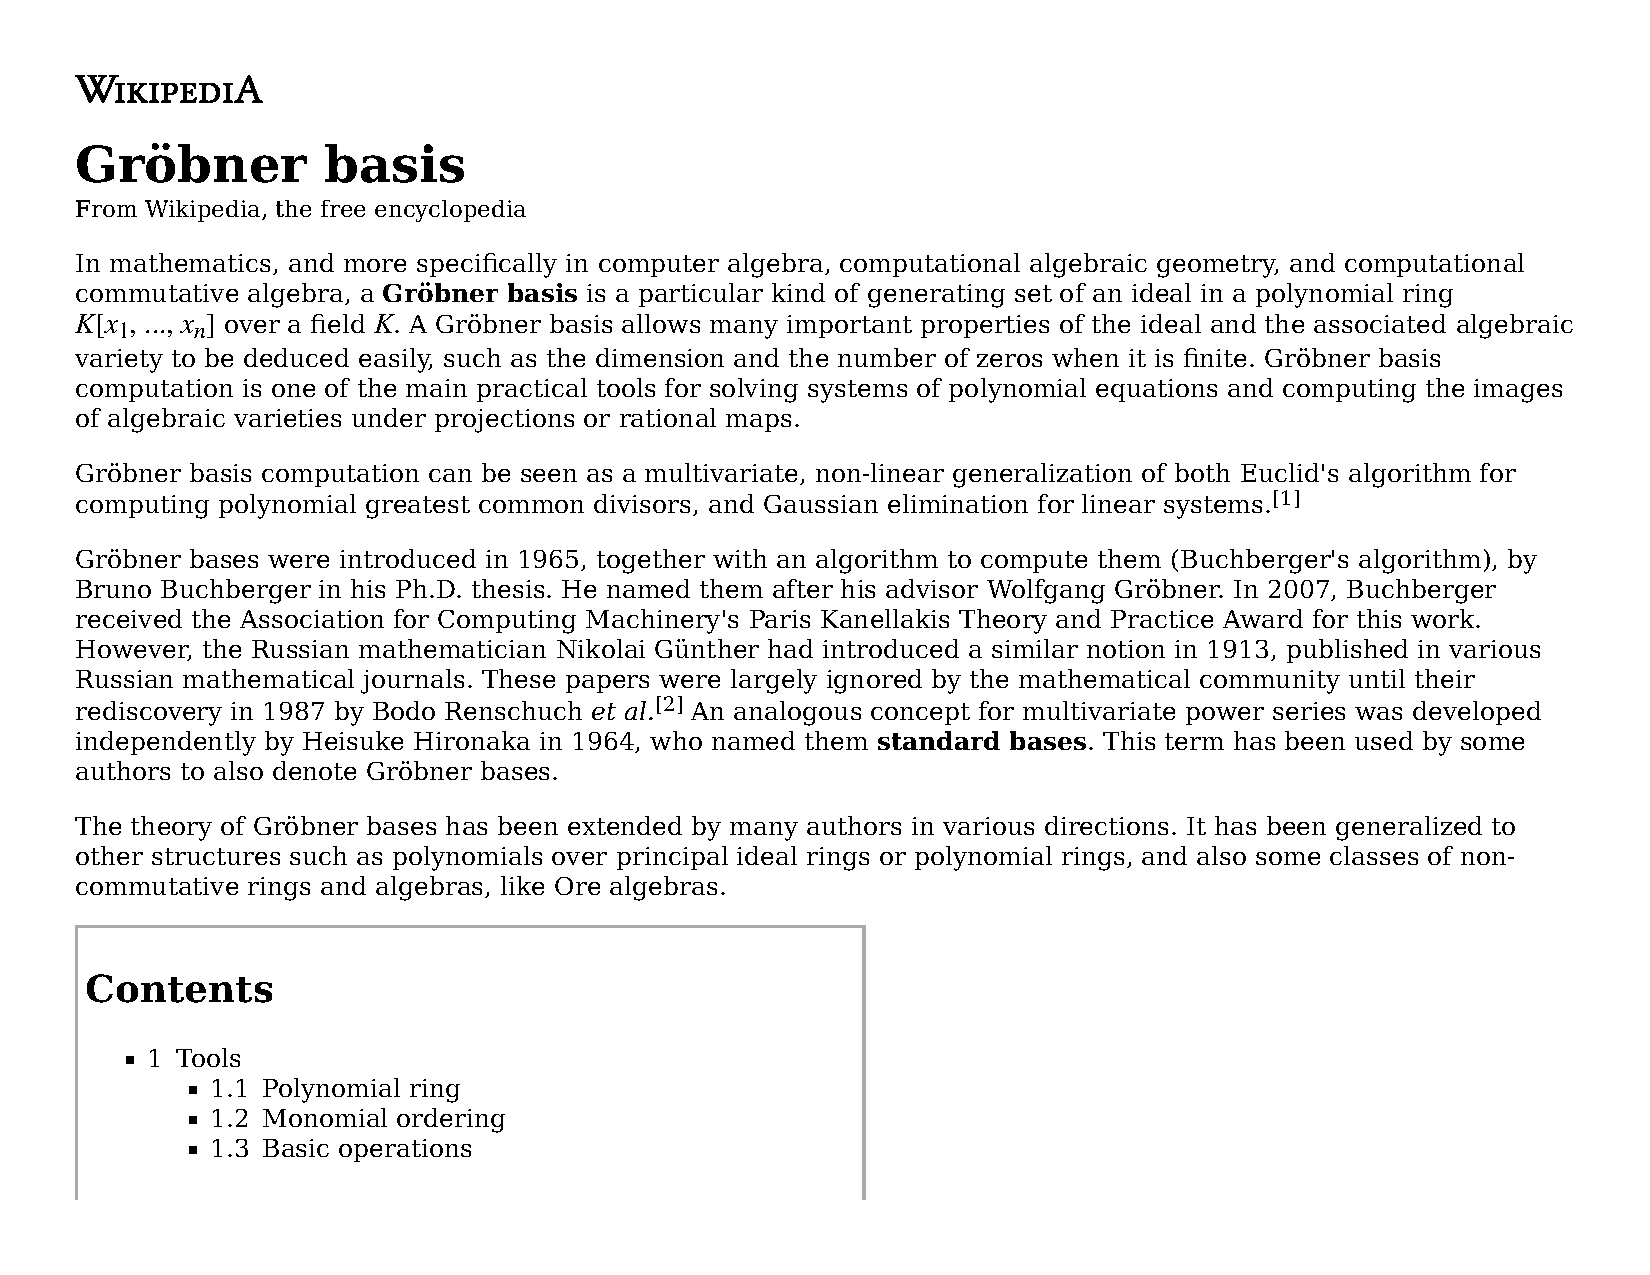
\includegraphics[clip, trim=0in 5.6in 0in 0.75in, width=\textwidth, page=1]{GrobnerBasis.pdf}
\includegraphics[clip, trim=0in 6.25in 0in 0.5in, width=\textwidth, page=9]{GrobnerBasis.pdf}
\includegraphics[clip, trim=0in 3in 0in 0.5in, width=\textwidth, page=13]{GrobnerBasis.pdf}
\end{frame}

\begin{frame}
\frametitle{Prof. Levin's Lagrange multipliers problem}
\includegraphics[page=29, clip, trim=0in 0in 2in 0in, width=\textwidth]{Levin-GB-Talk at CUA.pdf}
\end{frame}

\begin{frame}
\begin{semiverbatim}
\textcolor{blue}{sage:} R.<x,y,z,l> = PolynomialRing(QQ, order='lex')

\textcolor{blue}{sage:} f = x\^{}3 + 2*x*y*z - z\^{}2

\textcolor{blue}{sage:} g = x\^{}2 + y\^{}2 + z\^{}2 - 1

\textcolor{blue}{sage:} I = ideal([R(diff(f+l*g, v)) for v in (x,y,z,l)])

\textcolor{blue}{sage:} I.groebner\_basis()

$[x + y z + \frac{352}{221} l^{5} - \frac{10604}{3315} l^{4} - \frac{1596}{1105} l^{3} + \frac{7953}{1105} l^{2} - \frac{13747}{3315} l,$

$\allowbreak y^{2} + \frac{4448}{3315} l^{5} - \frac{22556}{9945} l^{4} - \frac{25232}{9945} l^{3} + \frac{55171}{9945} l^{2} - \frac{1198}{1105} l - 1,$

$y z l - y z - \frac{432}{1105} l^{5} + \frac{1398}{1105} l^{4} + \frac{6}{1105} l^{3} - \frac{6291}{2210} l^{2} + \frac{4347}{2210} l,$

$y l^{2} - y l - \frac{1}{5} z l^{2} - \frac{1}{5} z l + \frac{2}{5} z,$

$z^{2} - \frac{192}{221} l^{5} + \frac{1928}{1105} l^{4} + \frac{2076}{1105} l^{3} - \frac{4338}{1105} l^{2} + \frac{189}{1105} l,$

$z l^{3} - \frac{53}{24} z l^{2} + \frac{25}{24} z l + \frac{1}{6} z,$

$l^{6} - \frac{53}{24} l^{5} - \frac{29}{24} l^{4} + \frac{493}{96} l^{3} - \frac{75}{32} l^{2} - \frac{3}{8} l]$

\textcolor{blue}{sage:} I.groebner\_basis()[-1])

$l^{6} - \frac{53}{24} l^{5} - \frac{29}{24} l^{4} + \frac{493}{96} l^{3} - \frac{75}{32} l^{2} - \frac{3}{8} l$

\textcolor{blue}{sage:} I.groebner\_basis()[-1].numerator()

$96 l^{6} - 212 l^{5} - 116 l^{4} + 493 l^{3} - 225 l^{2} - 36 l$

\textcolor{blue}{sage:} I.groebner\_basis()[-1].numerator().factor()

$l \cdot (l - 1) \cdot (2 l - 3) \cdot (2 l + 3) \cdot (3 l - 4) \cdot (8 l + 1)$

\end{semiverbatim}
\end{frame}

\begin{frame}
\begin{semiverbatim}
\textcolor{blue}{sage:} I.variety()

$[\text{\texttt{{\char`\{}l:{ }0,{ }z:{ }0,{ }y:{ }1,{ }x:{ }0{\char`\}}}},
\break\text{\texttt{{\char`\{}l:{ }0,{ }z:{ }0,{ }y:{ }{-}1,{ }x:{ }0{\char`\}}}},
\break\text{\texttt{{\char`\{}l:{ }1,{ }z:{ }1,{ }y:{ }0,{ }x:{ }0{\char`\}}}},
\break\text{\texttt{{\char`\{}l:{ }1,{ }z:{ }{-}1,{ }y:{ }0,{ }x:{ }0{\char`\}}}},
\break\text{\texttt{{\char`\{}l:{ }3/2,{ }z:{ }0,{ }y:{ }0,{ }x:{ }{-}1{\char`\}}}},
\break\text{\texttt{{\char`\{}l:{ }{-}3/2,{ }z:{ }0,{ }y:{ }0,{ }x:{ }1{\char`\}}}},
\break\text{\texttt{{\char`\{}l:{ }4/3,{ }z:{ }2/3,{ }y:{ }1/3,{ }x:{ }{-}2/3{\char`\}}}},
\break\text{\texttt{{\char`\{}l:{ }4/3,{ }z:{ }{-}2/3,{ }y:{ }{-}1/3,{ }x:{ }{-}2/3{\char`\}}}}]$


\textcolor{blue}{sage:} [f.subs(dict(pt)) for pt in I.variety()]

$\left[0, 0, -1, -1, -1, 1, -\frac{28}{27}, -\frac{28}{27}\right]$


\end{semiverbatim}
\end{frame}

\begin{frame}[fragile]
\frametitle{Lagrange multipliers done correctly with {\tt QQbar}}
\begin{semiverbatim}
\textcolor{blue}{sage:} R.<x,y,z,l> = PolynomialRing(QQbar, order='lex') 
....: f = x^3 + 2*x*y*z - z^2 
....: g = x^2 + y^2 + z^2 - 1 
....: I = ideal([R(diff(f+l*g, v)) for v in (x,y,z,l)]) 
....: I.variety()                                                                                                                  
[{l: 0, z: 0, y: 1, x: 0},
 {l: 0, z: 0, y: -1, x: 0},
 {l: 1, z: 1, y: 0, x: 0},
 {l: 1, z: -1, y: 0, x: 0},
 {l: 3/2, z: 0, y: 0, x: -1},
 {l: -3/2, z: 0, y: 0, x: 1},
 {l: 4/3, z: 2/3, y: 1/3, x: -2/3},
 {l: 4/3, z: -2/3, y: -1/3, x: -2/3},
 {l: -1/8, z: -1/8*sqrt(11/2), y: 3/8*sqrt(11/2), x: -3/8},
 {l: -1/8, z: 1/8*sqrt(11/2), y: -3/8*sqrt(11/2), x: -3/8}]
\textcolor{blue}{sage:} [f.subs(dict(pt)) for pt in I.variety()]
[0, 0, -1, -1, -1, 1, -28/27, -28/27, 7/128, 7/128]

\end{semiverbatim}
\end{frame}

\begin{frame}[fragile]
\frametitle{The Lagrange multipliers problem done with Bertini}
The Bertini input file
\begin{semiverbatim}\small
CONFIG

END;

INPUT

variable_group x, y, z, l;
function f, g, h, i;

f = 3*x^2 + 2*x*l + 2*y*z;
g = 2*x*z + 2*y*l;
h = 2*x*y + 2*z*l + (-2)*z;
i = x^2 + y^2 + z^2 - 1;

END;
\end{semiverbatim}
\end{frame}

\begin{frame}[fragile]
\frametitle{The Lagrange multipliers problem done with Bertini}
The {\tt finite\_solutions} output file
\begin{semiverbatim}\tiny
12                                               

-6.666666666666669e-01 -1.387778780781446e-16
3.333333333333327e-01 -2.081668171172169e-16
6.666666666666657e-01 -1.942890293094024e-16
1.333333333333333e+00 1.110223024625157e-16

-1.242639553753176e-15 1.037232314986088e-15
-1.086567340276065e-15 1.755622365349657e-15
-9.999999999999994e-01 3.434752482434078e-16
1.000000000000000e+00 7.068998164605489e-16

...

0.640708586058897743697e-14 -0.312021282000262752677e-14
-0.142713225653312452193e-14 0.479093022537473430205e-14
0.100000000000000442723e1 0.347026010358297831715e-15
0.100000000000000125811e1 0.443850685372115805194e-14

0.568153222086140476406e-14 -0.395514379958853185339e-14
-0.822128696941474670143e-15 0.554792978704183544098e-14
0.999999999999999876672e0 -0.871590126461097014499e-15
0.999999999999999884261e0 0.498793985715534349268e-14

-3.750000000000001e-01 -5.551115123125783e-17
-8.794529549668934e-01 0.000000000000000e+00
2.931509849889644e-01 6.938893903907228e-18
-1.250000000000000e-01 -8.673617379884035e-17

\end{semiverbatim}
\end{frame}

\begin{frame}[fragile]
\frametitle{Exactness recovery with {\tt ries}}
\begin{exampleblock}{{\tt http://mrob.com/pub/ries/index.html}}
ries (or RIES, an acronym for RILYBOT Inverse Equation Solver) takes any number and produces a list of equations that approximately solve to that number.
\end{exampleblock}
\begin{semiverbatim}\tiny
$ ries -a 2.931509849889644e-01

   Your target value: T = 0.293150984988964                      mrob.com/ries

                    9 x = phi^2                  for x = T - 0.00225832  {65}
                    9 x = sqrt(7)                for x = T + 0.000821383 {65}
                1/(x-1) = -sqrt(2)               for x = T - 0.000257766 {66}
                  1/x-3 = 1/sqrt(6)              for x = T + 0.000254869 {76}
                  x-1/3 = 1/-(5^2)               for x = T + 0.000182348 {82}
            x+sqrt(phi) = 4"/6                   for x = T - 8.60544e-05 {87}
                (8 x)^2 = 1/2+5                  for x = T - 5.55112e-17 {88}
  (Stopping now because best match is within   1e-15 of target value.)

  phi = the golden ratio, (1+sqrt(5))/2  sqrt(x) = square root
  A"/B = Ath root of B

                         --LHS--      --RHS--      -Total-
     max complexity:          47           42           89
          dead-ends:        8883        17840        26723  Time: 0.006
        expressions:         484          838         1322
           distinct:         373          386          759  Memory: 57392 B

        Total equations tested:                  143978 (1.44e+05)
\end{semiverbatim}
\end{frame}

\begin{frame}[fragile]
\frametitle{The Lagrange multipliers problem done with Bertini}
\begin{semiverbatim}
\end{semiverbatim}
\end{frame}

\begin{frame}[fragile]
\frametitle{Prof. Levin's graph coloring problem}
Can this graph be 3-colored?
\vskip 20pt
\includegraphics[page=32, clip, trim=0in 0in 2in 3.5in, width=\textwidth]{Levin-GB-Talk at CUA.pdf}
\end{frame}

\begin{frame}[fragile]
\frametitle{Bertini - {\tt bertini.nd.edu}}
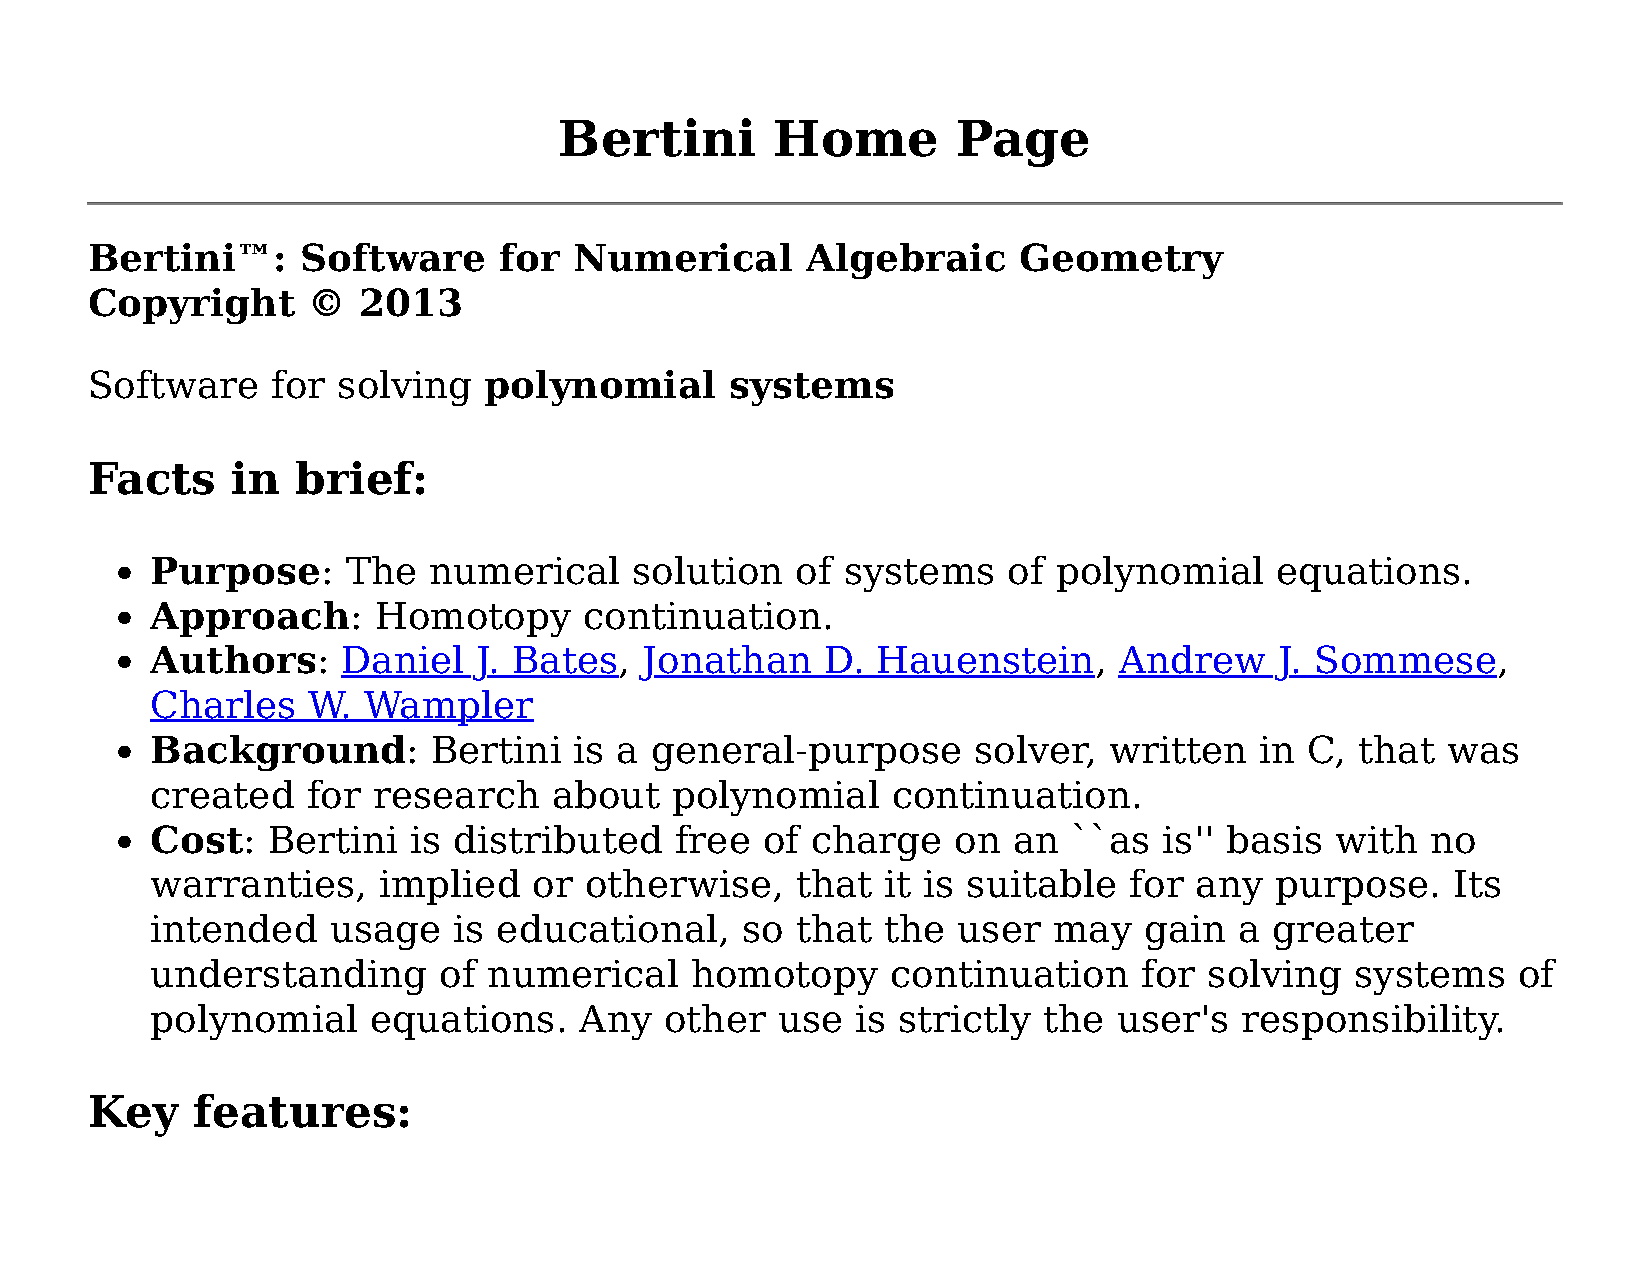
\includegraphics[page=1, clip, trim=0in 1.5in 0in 0in, width=\textwidth]{bertini.nd.edu.pdf}
\end{frame}

\begin{frame}

\begin{semiverbatim}
\scriptsize
\textcolor{blue}{sage:} R=PolynomialRing(QQ, names=[f'x\{i\}' for i in range(1,9)], order='lex')

\textcolor{blue}{sage:} edges = [(1,2), (1,5), (1,6), (2,3), (2,4), (2,8),

\ \ \ \ \ \ \ \ \ \ \ \ \ \ \        (3,4), (3,8), (4,5), (4,7), (5,6), (6,7), (7,8)]


\textcolor{blue}{sage:} set1 = [g\^{}3 - 1 for g in R.gens()]

$\left[x_{1}^{3} - 1, x_{2}^{3} - 1, x_{3}^{3} - 1, x_{4}^{3} - 1, x_{5}^{3} - 1, x_{6}^{3} - 1, x_{7}^{3} - 1, x_{8}^{3} - 1\right]$


\textcolor{blue}{sage:} set2 = [R.gen(i-1)\^{}2 + R.gen(i-1)*R.gen(j-1) + R.gen(j-1)\^{}2 for i,j in edges]
$[x_{1}^{2} + x_{1} x_{2} + x_{2}^{2}, x_{1}^{2} + x_{1} x_{5} + x_{5}^{2}, x_{1}^{2} + x_{1} x_{6} + x_{6}^{2}, x_{2}^{2} + x_{2} x_{3} + x_{3}^{2}, x_{2}^{2} + x_{2} x_{4} + x_{4}^{2}, x_{2}^{2} + x_{2} x_{8} + x_{8}^{2},$

$x_{3}^{2} + x_{3} x_{4} + x_{4}^{2}, x_{3}^{2} + x_{3} x_{8} + x_{8}^{2}, x_{4}^{2} + x_{4} x_{5} + x_{5}^{2}, x_{4}^{2} + x_{4} x_{7} + x_{7}^{2}, x_{5}^{2} + x_{5} x_{6} + x_{6}^{2}, x_{6}^{2} + x_{6} x_{7} + x_{7}^{2}, x_{7}^{2} + x_{7} x_{8} + x_{8}^{2}]$

\textcolor{blue}{sage:} I=R.ideal(set1 + set2)

\textcolor{blue}{sage:} I.groebner\_basis()

$[x_{1} + x_{5} + x_{6}, x_{2} + x_{3} + x_{8}, x_{3}^{2} + x_{3} x_{8} + x_{8}^{2}, x_{3} x_{5} - x_{3} x_{7} - x_{5} x_{7} - x_{7} x_{8} - x_{8}^{2},$

$x_{3} x_{6} + x_{3} x_{7} + x_{3} x_{8} + x_{5} x_{7} + 2 x_{5} x_{8} + x_{6} x_{7} + x_{6} x_{8} + x_{8}^{2}, x_{4} - x_{8}, x_{5}^{2} + x_{5} x_{8} + x_{8}^{2},$

$x_{5} x_{6} - x_{5} x_{8} - x_{6} x_{7} + x_{7} x_{8}, x_{6}^{2} + x_{6} x_{7} - x_{7} x_{8} - x_{8}^{2}, x_{7}^{2} + x_{7} x_{8} + x_{8}^{2}, x_{8}^{3} - 1]$

\textcolor{blue}{sage:} I.variety()

[]



\textcolor{blue}{sage:} R=PolynomialRing(QQbar, names=[f'x\{i\}' for i in range(1,9)], order='lex')

\textcolor{blue}{sage:} set1 = [g\^{}3 - 1 for g in R.gens()]

\textcolor{blue}{sage:} set2 = [R.gen(i-1)\^{}2 + R.gen(i-1)*R.gen(j-1) + R.gen(j-1)\^{}2 for i,j in edges]

\textcolor{blue}{sage:} I = R.ideal(set1 + set2)

\textcolor{blue}{sage:} I.groebner\_basis()

\textcolor{blue}{sage:} I.variety()

\textcolor{blue}{sage:} QQbar.options.display\_format = 'radical'

\textcolor{blue}{sage:} len(I.variety())

8

\textcolor{blue}{sage:} I.variety()[0]

$\text{\texttt{{\char`\{}x8:{ }1,{ }x7:{ }{-}1/2*I*sqrt(3){ }{-}{ }1/2,{ }x6:{ }1,{ }x5:{ }{-}1/2*I*sqrt(3){ }{-}{ }1/2,{ }x4:{ }1,{ }x3:{ }1/2*I*sqrt(3){ }{-}{ }1/2,{ }x2:{ }{-}1/2*I*sqrt(3){ }{-}{ }1/2,{ }x1:{ }1/2*I*sqrt(3){ }{-}{ }1/2{\char`\}}}}$

\end{semiverbatim}


\end{frame}

\begin{frame}

\begin{exampleblock}{Learning a performance metric of Buchberger's algorithm

Jelena Mojsilovi\'c, Dylan Peifer, Sonja Petrovi\'c ({\tt arxiv.org}, 2021)
}
Many computer algebra systems offer generic algorithms for computing Gr\"obner bases
applicable to all kinds of input ideals. In the 1960s, Buchberger developed a groundbreaking
algorithm [Buchberger, 2006] to compute a Gr\"obner basis of any ideal, a problem that is
NP-hard in general. As it applies to any polynomial system, Buchberger's algorithm has a
doubly exponential runtime in the number of variables [Dube, 1990]. In the decades that followed,
several specialized algorithms have been used to improve runtime: Belt\'ran and Pardo
[2008, 2009.], Cox et al. [2007]. These algorithms form the cornerstone of the field of symbolic
computational nonlinear algebra.
\end{exampleblock}

\end{frame}

\begin{frame}
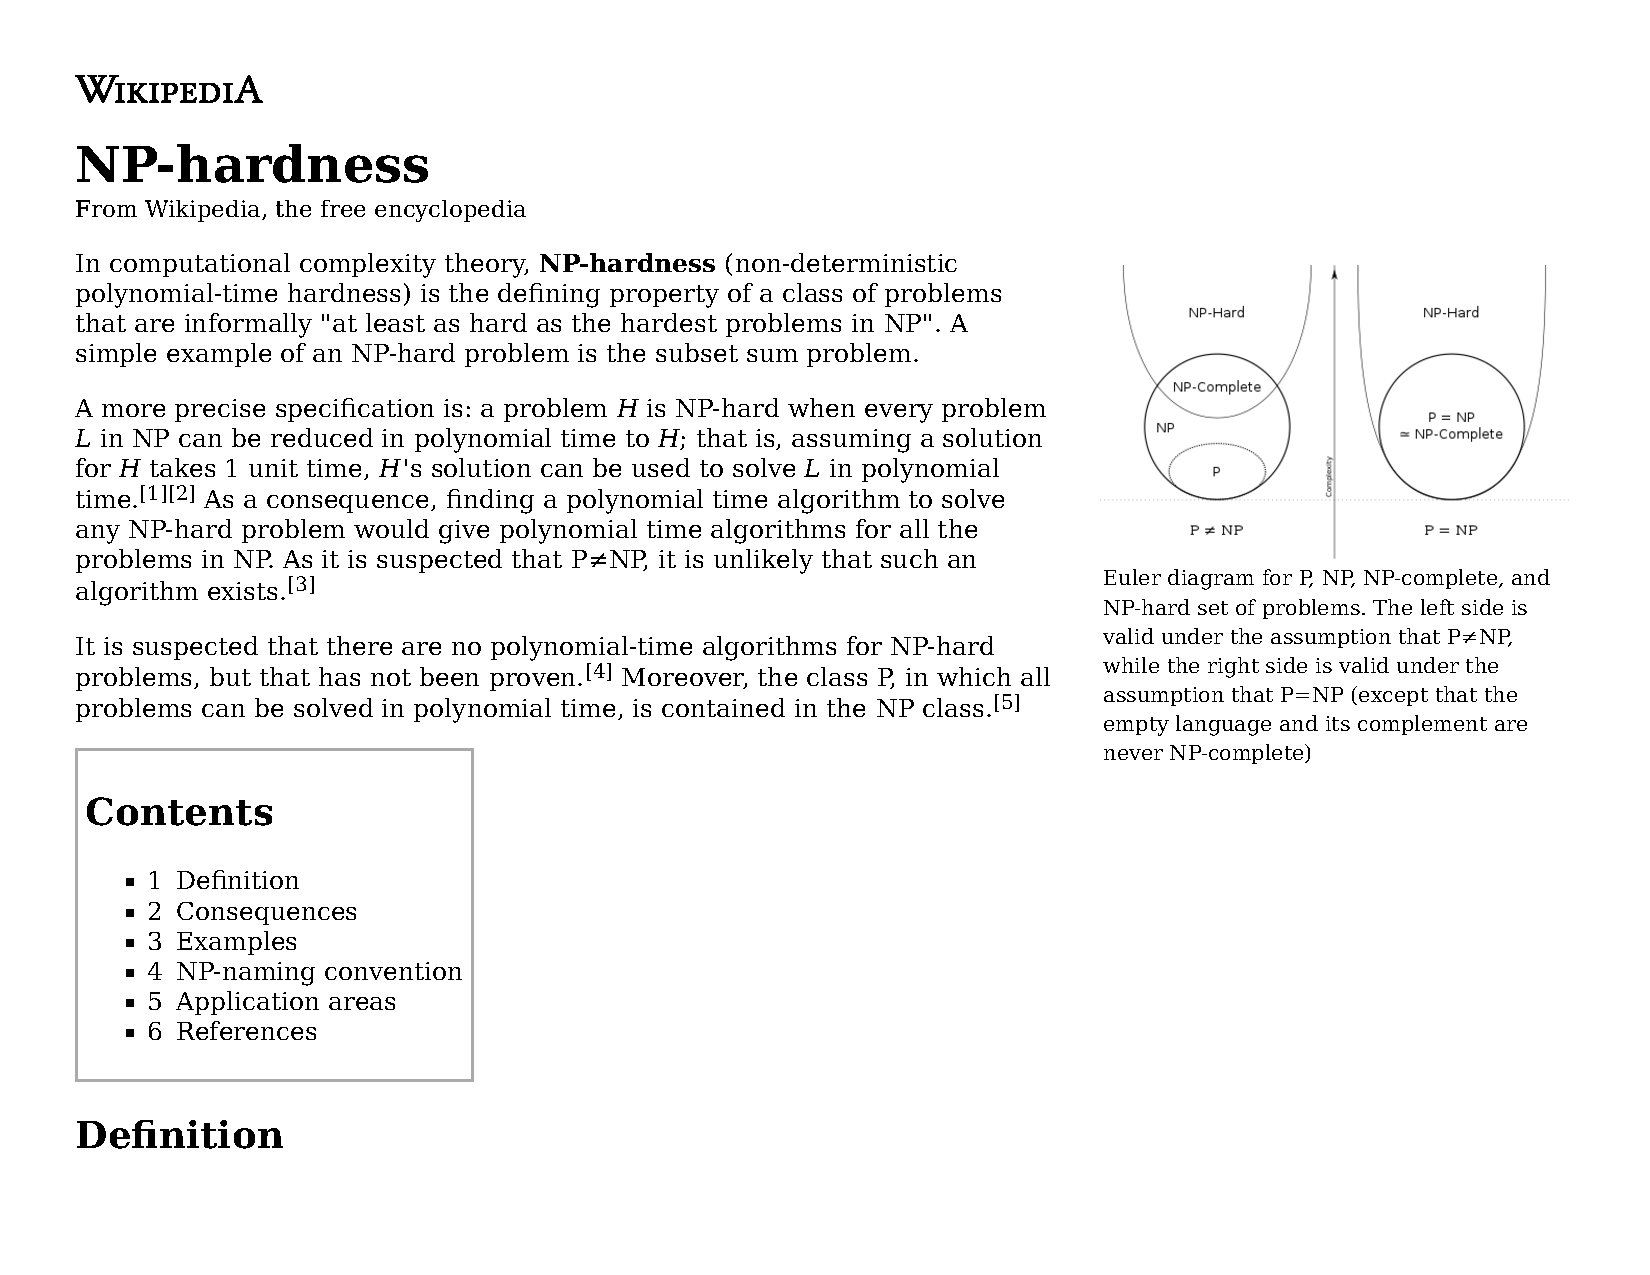
\includegraphics[width=\textwidth]{NP-hardness - Wikipedia.pdf}
\end{frame}

\begin{frame}

\begin{exampleblock}{Learning a performance metric of Buchberger's algorithm

Jelena Mojsilovi\'c, Dylan Peifer, Sonja Petrovi\'c ({\tt arxiv.org}, 2021)
}
Improvements on Buchberger's algorithm, such as Faug\'ere's famous F5 algorithm developed
in Faug\'ere et al. [1993], Faug\'ere et al. [2014], leverage the fact that the computation is
a generalization of Gaussian elimination. As such, these methods construct nontrivial
organizational techniques, such as cleverly organizing monomials into large matrices, to judiciously
perform Buchberger's key step: reduction of S-polynomials. Namely, the algorithm grows a
given generating set by adding nonzero remainders of S-polynomials upon division by the
current generating set; an S-polynomial is an element of the ideal created from a pair of
given polynomials. The correctness of Buchberger's algorithm does not depend on the order
in which such pairs, called S-pairs, are processed: one can simply create all pairs, store them
in a queue in arbitrary order, and process them linearly. On the other hand, the above
mentioned algorithms indicate – and by now this is part of the computational nonlinear algebra
folklore – one can improve the runtime by reorganizing the polynomials in the generating set
so as to process the S-pairs in different order.
%Standard strategies select pairs based on some
%minimality criterion, such as the degree of the least common multiple of the two leading terms
%or its position in the monomial order.
\end{exampleblock}

\end{frame}

\begin{frame}

\begin{exampleblock}{Learning a performance metric of Buchberger's algorithm

Jelena Mojsilovi\'c, Dylan Peifer, Sonja Petrovi\'c ({\tt arxiv.org}, 2021)
}
Within the paradigm of using
learning to improve algorithms that give the exact answer, Peifer et al. [2020] uses machine
learning to discover new S-pair selection strategies in Buchberger's algorithm which outperform
state-of-the-art human-designed heuristics by 20\% to 40\%. Their main contribution was
to express S-pair selection in Buchberger's algorithm as a reinforcement learning problem, i.e.
a game where the player or agent selects S-pairs and is rewarded for minimizing the overall
computational cost of the algorithm. Their measure of computational cost was the number
of polynomial additions performed, which is a hardware- independent number that indicates
how hard the basis was to compute.
\end{exampleblock}

\end{frame}

\begin{frame}

\begin{exampleblock}{Learning a performance metric of Buchberger's algorithm

Jelena Mojsilovi\'c, Dylan Peifer, Sonja Petrovi\'c ({\tt arxiv.org}, 2021)
}
A key part of many reinforcement learning techniques
is a value model which learns to predict future reward...
such a model would predict the number of future polynomial
additions before the Gr\"obner basis computation is complete. The goal of this manuscript is
to learn a version of this value function in the supervised learning setting
\end{exampleblock}

\begin{exampleblock}{}
JM is a PhD student at Purdue University. SP is with Illinois Tech's Applied Math Department, and
partially supported by the Simons Foundation Collaboration Grant for Mathematicians 854770. At the time
of the first version of this manuscript, JM was an Applied Math undergraduate researcher at Illinois Tech and
DP was a Mathematics PhD student at Cornel
\end{exampleblock}

\end{frame}

\begin{frame}
\begin{itemize}
\item alternatives: numerical techniques
\item witness points: approximate solutions accurate enough to find exact solutions
\item LLL algorithm

\item Andrew Sommese - Notre Dame

Daniel J. Bates, Jonathan D. Hauenstein, Timothy M. McCoy, Chris Peterson \& Andrew J. Sommese (2013)
Recovering Exact Results from Inexact Numerical Data in Algebraic Geometry,
Experimental Mathematics, 22:1, 38-50, DOI: 10.1080/10586458.2013.737640

\item "exactness recovery algorithms"
\item https://en.wikipedia.org/wiki/Lenstra%E2%80%93Lenstra%E2%80%93Lov%C3%A1sz_lattice_basis_reduction_algorithm

\item Newton's method
     {\tt https://en.wikipedia.org/wiki/File:NewtonIteration\_Ani.gif}

\item Bertini's homotopy continuation method
\item {\tt https://en.wikipedia.org/wiki/Homotopy}
\end{itemize}
\end{frame}

\begin{frame}
\frametitle{Hybrid numerical/symbolic techniques}
\begin{itemize}
\item Gr\"obner bases are computed using exact (integer) arithmetic
\item The obvious alternative: a numerical technique, but we lose exactness (or do we?)
\item {\it Witness points} are approximate solutions accurate enough to find exact solutions
\item "Exactness recovery algorithms" such as LLL
\end{itemize}

\end{frame}

\begin{frame}
\begin{semiverbatim}
\small
x = 0.464918758265008

y = 0.5179110625786596

z = 0.7180659297529489



L = [a for a in (1,x,y,z,x\^{}2,y\^{}2,z\^{}2,x*y,x*z,y*z)]


$\begin{array}{r}
1.00000000000000 \\
0.464918758265008 \\
0.517911062578660 \\
0.718065929752949 \\
0.216149451786677 \\
0.268231868741356 \\
0.515618679471967 \\
0.240786568105781 \\
0.333842320413149 \\
0.371894288679883
\end{array}
$

\end{semiverbatim}
\end{frame}

\begin{frame}
\begin{semiverbatim}
\small

def lindepmat(L,N):

\ \ \ \ return matrix(ZZ,[[1 if i==j else 0

\ \ \ \ \ \ \ \ \ \ \ \ \ \   for i in [0..len(L)-1]] + [round(N*L[j])]

\ \ \ \ \ \ \ \ \ \ \ \ \ \   for j in [0..len(L)-1]])

{\tiny {\tt http://people.math.sfu.ca/\~{}summerschool/summer\_school\_2014/LLL\_sage\_computations.html}}



M = lindepmat(L,10\^{}13)


$\left(\begin{array}{rrrrrrrrrrr}
1 & 0 & 0 & 0 & 0 & 0 & 0 & 0 & 0 & 0 & 10000000000000 \\
0 & 1 & 0 & 0 & 0 & 0 & 0 & 0 & 0 & 0 & 4649187582650 \\
0 & 0 & 1 & 0 & 0 & 0 & 0 & 0 & 0 & 0 & 5179110625787 \\
0 & 0 & 0 & 1 & 0 & 0 & 0 & 0 & 0 & 0 & 7180659297529 \\
0 & 0 & 0 & 0 & 1 & 0 & 0 & 0 & 0 & 0 & 2161494517867 \\
0 & 0 & 0 & 0 & 0 & 1 & 0 & 0 & 0 & 0 & 2682318687414 \\
0 & 0 & 0 & 0 & 0 & 0 & 1 & 0 & 0 & 0 & 5156186794720 \\
0 & 0 & 0 & 0 & 0 & 0 & 0 & 1 & 0 & 0 & 2407865681058 \\
0 & 0 & 0 & 0 & 0 & 0 & 0 & 0 & 1 & 0 & 3338423204131 \\
0 & 0 & 0 & 0 & 0 & 0 & 0 & 0 & 0 & 1 & 3718942886799
\end{array}\right)
$

\end{semiverbatim}
\end{frame}


\begin{frame}
\begin{semiverbatim}
\small

M.LLL()


$\left(\begin{array}{rrrrrrrrrrr}
-1 & 0 & 0 & 0 & 1 & 1 & 1 & 0 & 0 & 0 & 1 \\
4 & -2 & -5 & -11 & -4 & -9 & 16 & -2 & 11 & -2 & -1 \\
2 & -3 & 3 & 3 & 0 & 9 & 5 & -3 & -9 & -15 & -14 \\
-7 & 1 & 11 & -3 & -6 & -1 & 2 & -17 & 5 & 16 & -3 \\
-2 & 14 & 4 & 3 & 4 & -8 & -6 & -17 & 7 & -7 & 9 \\
-2 & -4 & -5 & 11 & -10 & -17 & 12 & -16 & 1 & 7 & 12 \\
-14 & 12 & 20 & -2 & -7 & -1 & 3 & 4 & 3 & -6 & -10 \\
-4 & -13 & -3 & 18 & 6 & 4 & -12 & -12 & 15 & 1 & -3 \\
5 & -19 & 14 & 3 & 6 & -14 & 3 & -15 & 8 & -10 & 9 \\
11 & -11 & -1 & -1 & -20 & 12 & 6 & 3 & -2 & -18 & 12
\end{array}\right)$




\centerline{$-1 + x^2 + y^2 + z^2 = -10^{-13}$}

\centerline{$x^2 + y^2 + z^2 \approx 1$}


\end{semiverbatim}
\end{frame}

\begin{frame}
\begin{exampleblock}{Bates, Hauenstein, McCoy, Peterson, Sommese

Recovering Exact Results from Inexact Numerical Data in Algebraic Geometry,

Experimental Mathematics, 22:1, 38-50 (2013)}

Since the goal of this paper is the application of such methods rather than the
development of a new algorithm of this type, we will restrict our attention
to the LLL algorithm as described in [23, 17]. It is worth noting that there
are improvements to the LLL algorithm [26, 28, 27], as well as alternatives
(such as BKZ and PSLQ [16, 30]), but a full analysis and description of the
various options would not significantly enhance the value of this article.

By fixing the required input precision and the maximum degree of rela-
tions, it is clear that the above process terminates. It should be noted that
upper bounds do exist on the largest degree generator of P` given the degree
of the variety V (P`), see [9], but these tend to be impractically large. To
make matters worse, bounds on the coefficient size may not be known, and
hence the precision requirements may be ambiguous. While these issues can
be mitigated, as discussed in §2.4, they cannot at present be eliminated.

\end{exampleblock}

\end{frame}

\begin{frame}
\frametitle{Lenstra Lenstra Lov\'asz lattice basis reduction algorithm}
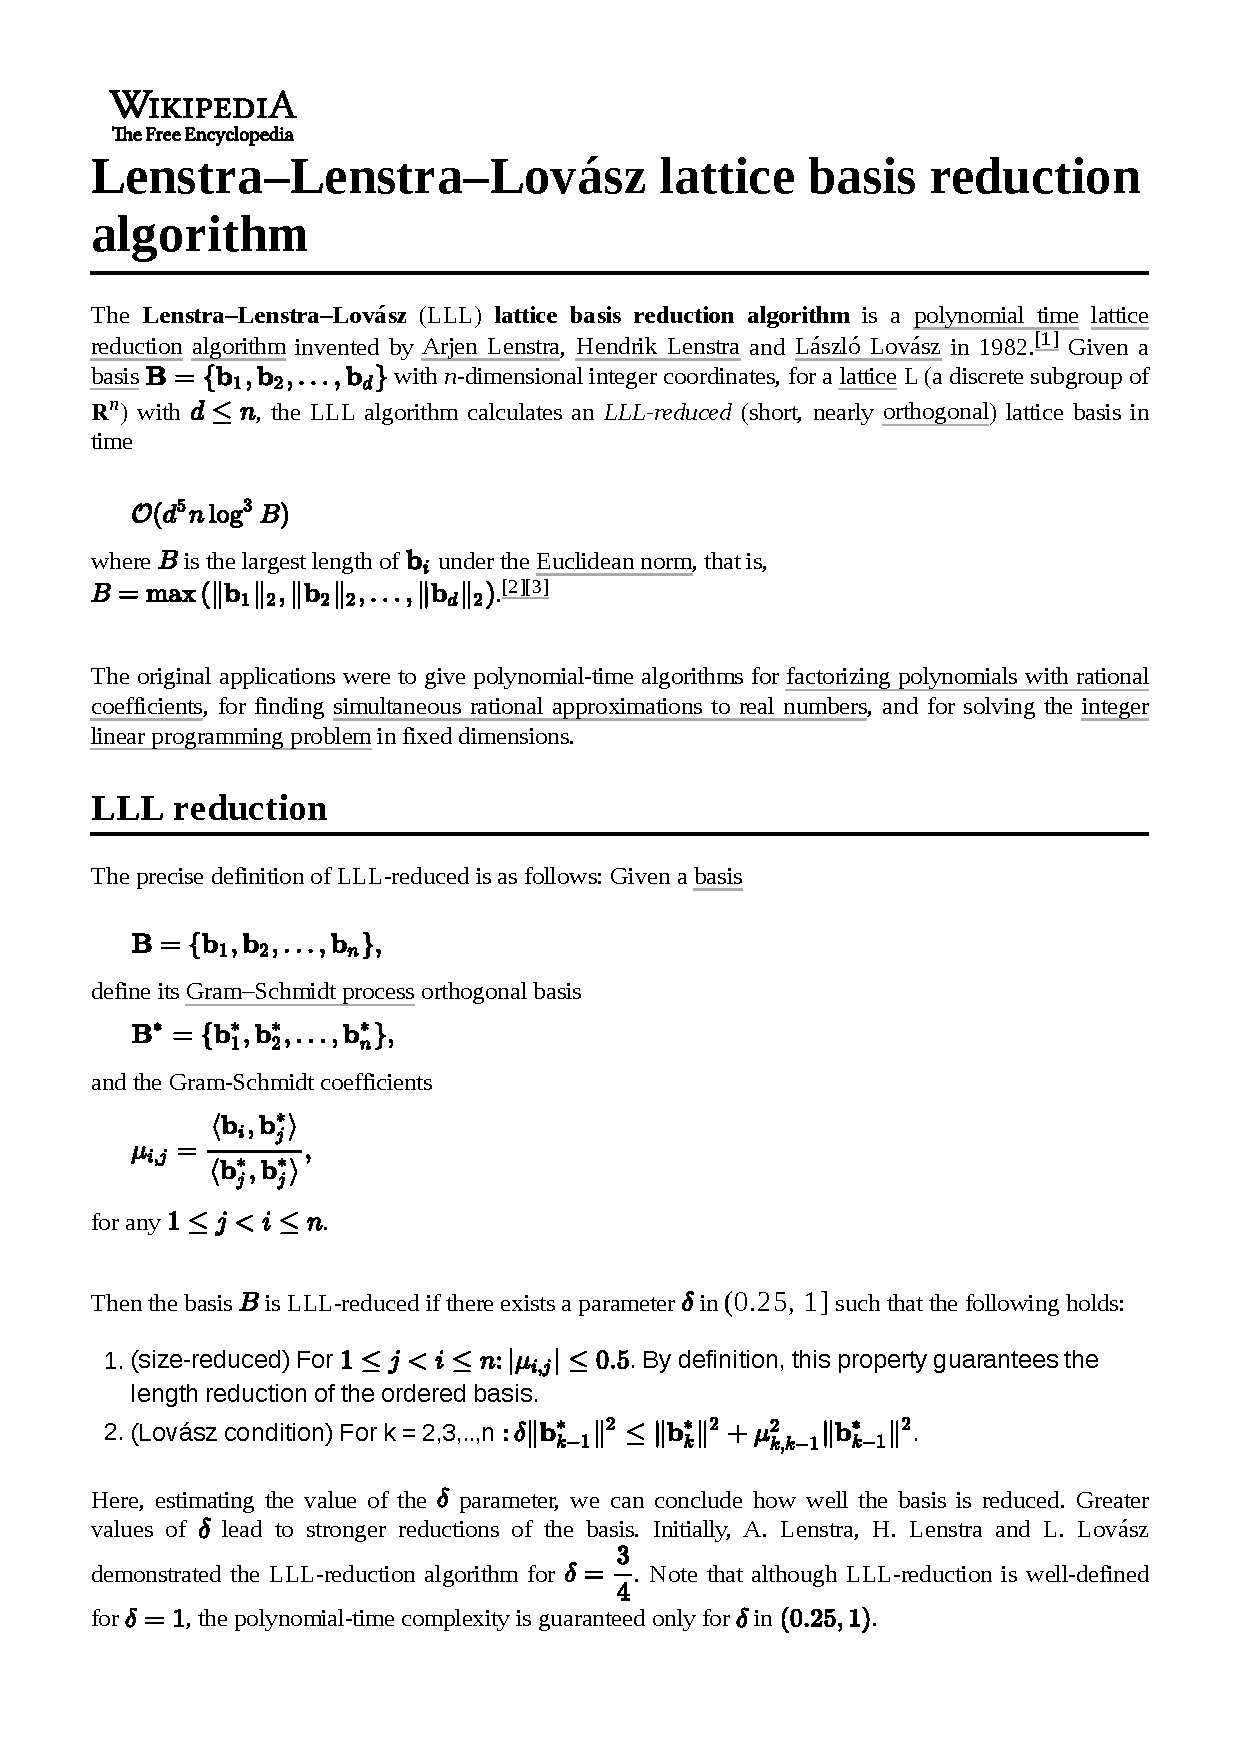
\includegraphics[page=1, clip, trim=0in 6.5in 0in 0in, width=\textwidth]{Lenstra–Lenstra–Lovasz_lattice_basis_reduction_algorithm.pdf}
\end{frame}

\begin{frame}
\frametitle{Lenstra Lenstra Lov\'asz lattice basis reduction algorithm}
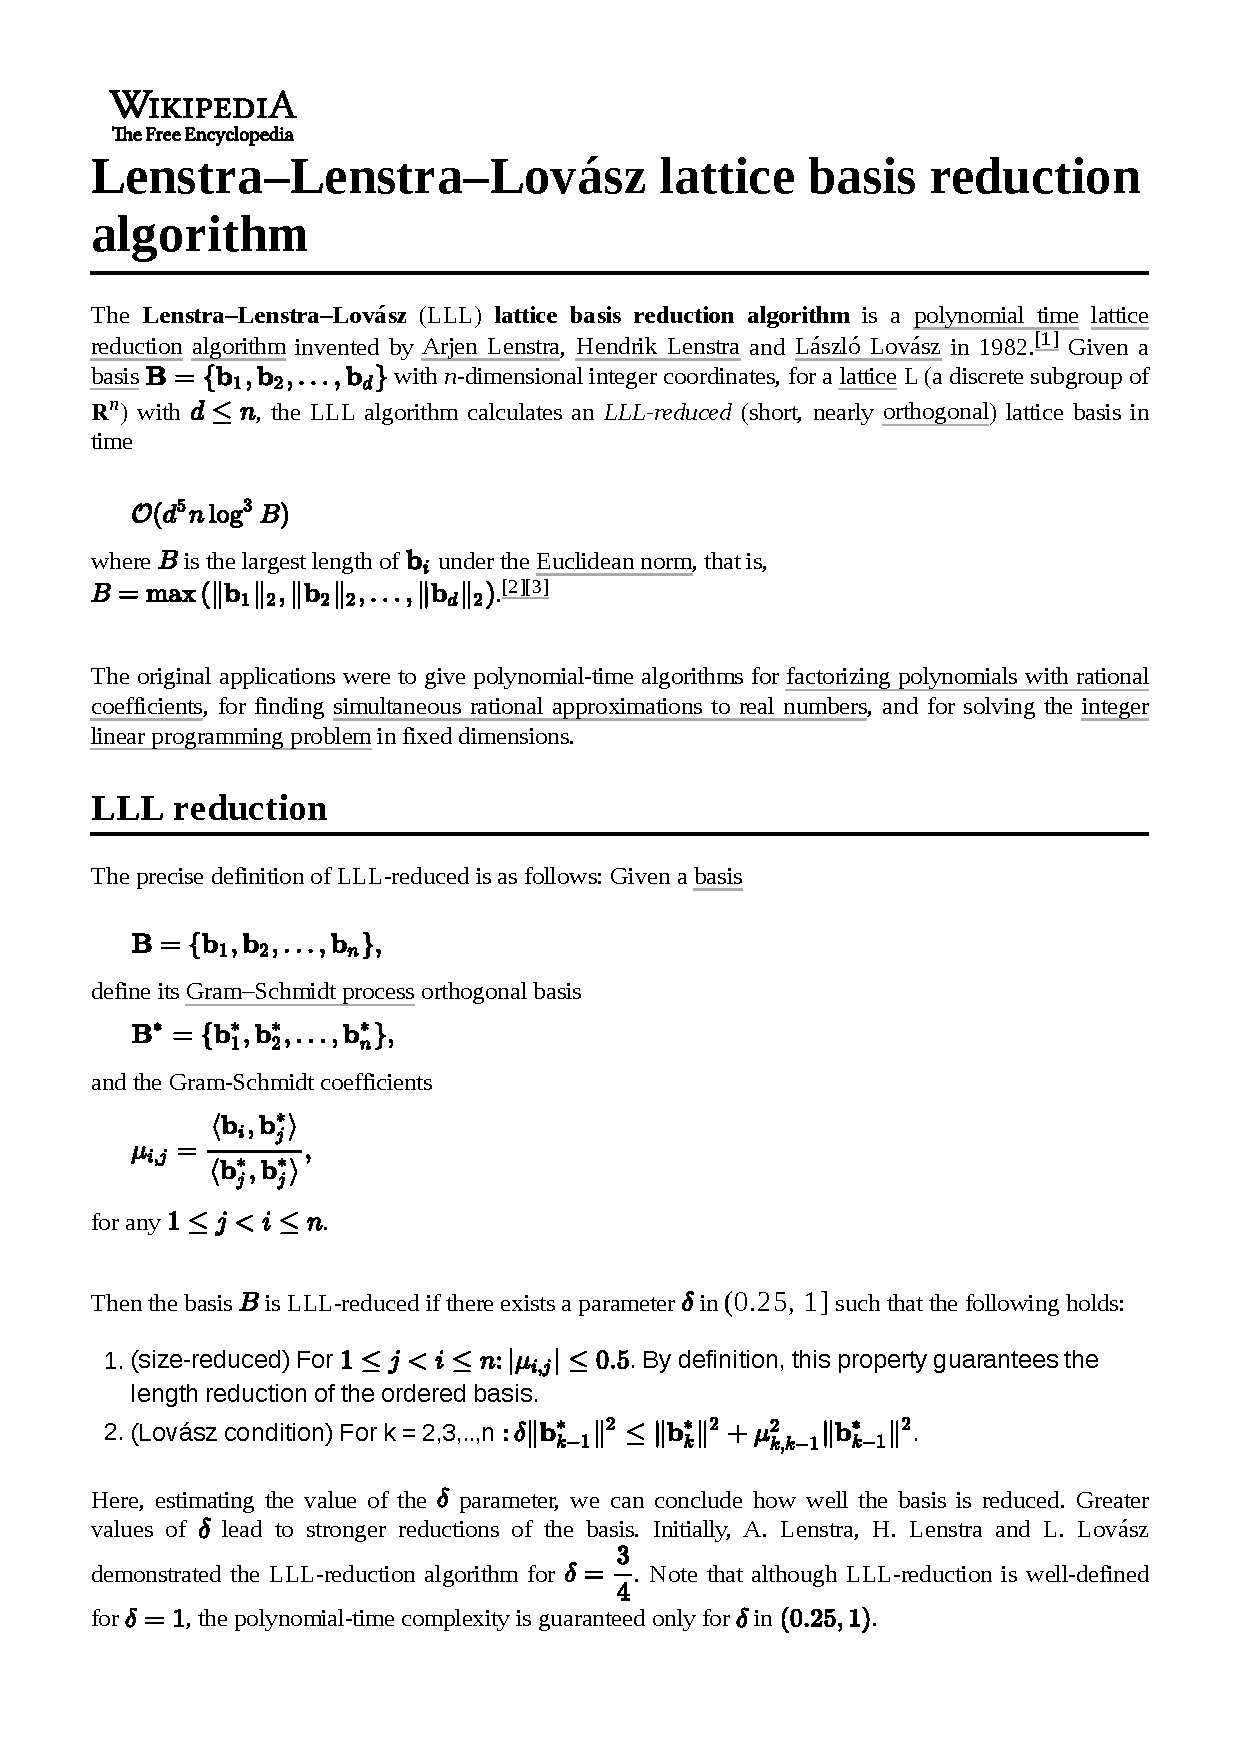
\includegraphics[page=1, clip, trim=0in 0in 0in 5in, width=\textwidth]{Lenstra–Lenstra–Lovasz_lattice_basis_reduction_algorithm.pdf}
\end{frame}

\begin{frame}
\frametitle{Lenstra Lenstra Lov\'asz lattice basis reduction algorithm}
\includegraphics[page=2,clip,trim=0in 0.8in 0in 9in, width=\textwidth]{Lenstra–Lenstra–Lovasz_lattice_basis_reduction_algorithm.pdf}
%\includegraphics[page=3,clip,trim=0in 11in 0in 0in, width=\textwidth]{Lenstra–Lenstra–Lovasz_lattice_basis_reduction_algorithm.pdf}
\includegraphics[page=3,clip,trim=0in 7.5in 0in 1in, width=\textwidth]{Lenstra–Lenstra–Lovasz_lattice_basis_reduction_algorithm.pdf}
\end{frame}

\begin{frame}
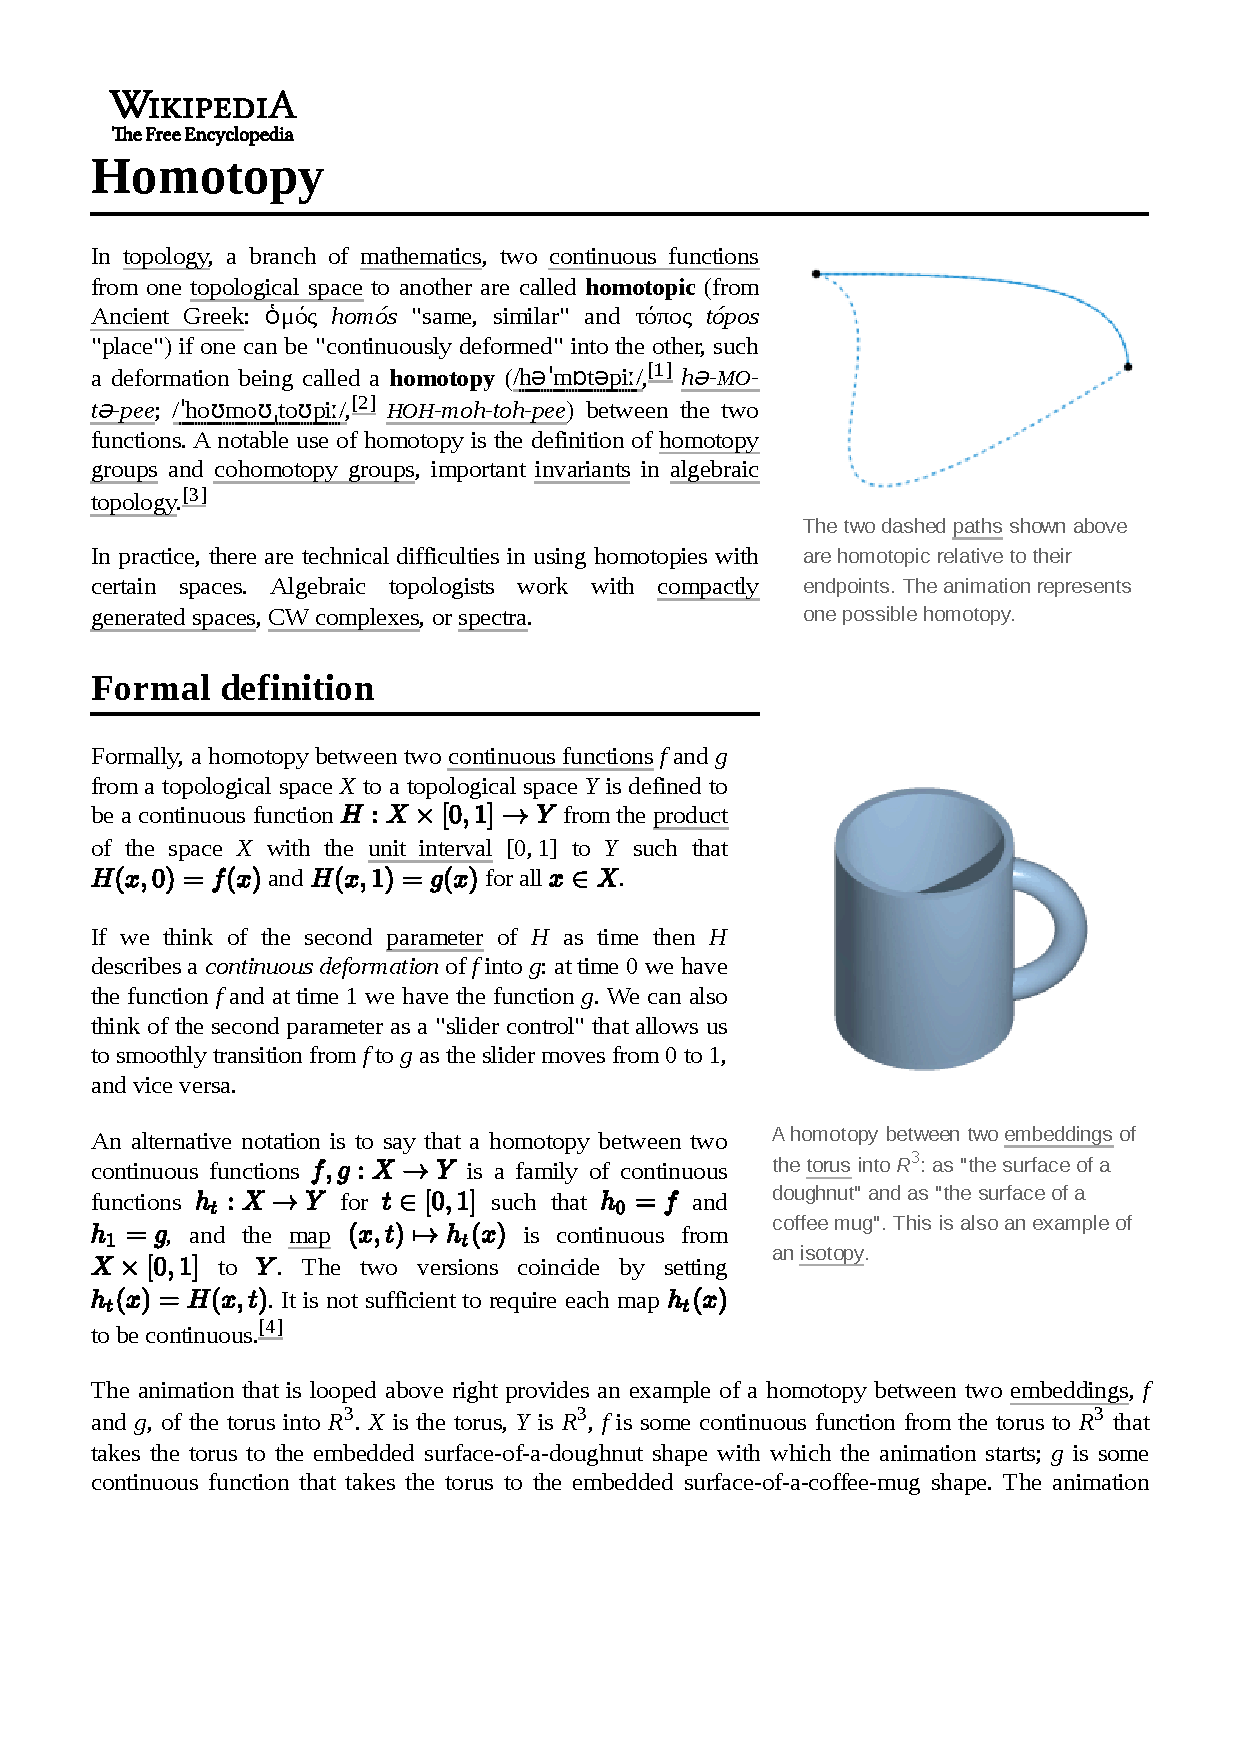
\includegraphics[width=\textwidth]{Homotopy.pdf}
\end{frame}

\begin{frame}
\begin{exampleblock}{}
\begin{center}
\vskip 20pt
\Huge
Part 2: Differential Algebra
\vskip 6pt
\ 
\end{center}
\end{exampleblock}
\end{frame}

\begin{frame}
\frametitle{Part 2}

\begin{itemize}
\item ASIDE: Rosenfeld-Grobner in differential algebra
\item my code: scipy's levenberg-marquet algorithm
\item my algorithm for fast evaluation of polynomials and Jacobians using sparse matrices
\item optimization: use shared memory to run computations in parallel
\item potential scipy optimization for parallel QR decomposition
\item potential scipy optimization for superscalar sparse multiplication
     types of matrix storage layouts: dense, sparse (COO, CSC, CSR, DOK)
%     csr_matvec in ~/src/scipy/scipy/sparse/sparsetools/csr.h

\item example: the f(x+r) solutions
\item show several examples, lattice reduction by hand, and demonstrate that it's a dot product
\item why it doesn't solve Schrodinger globally
\item using Kovacic's algorithm to determine that it's non-elementary
\item Mathematica says it's related to the Bessel functions
\item show how
\end{itemize}
\end{frame}

\begin{frame}
\frametitle{My Question}
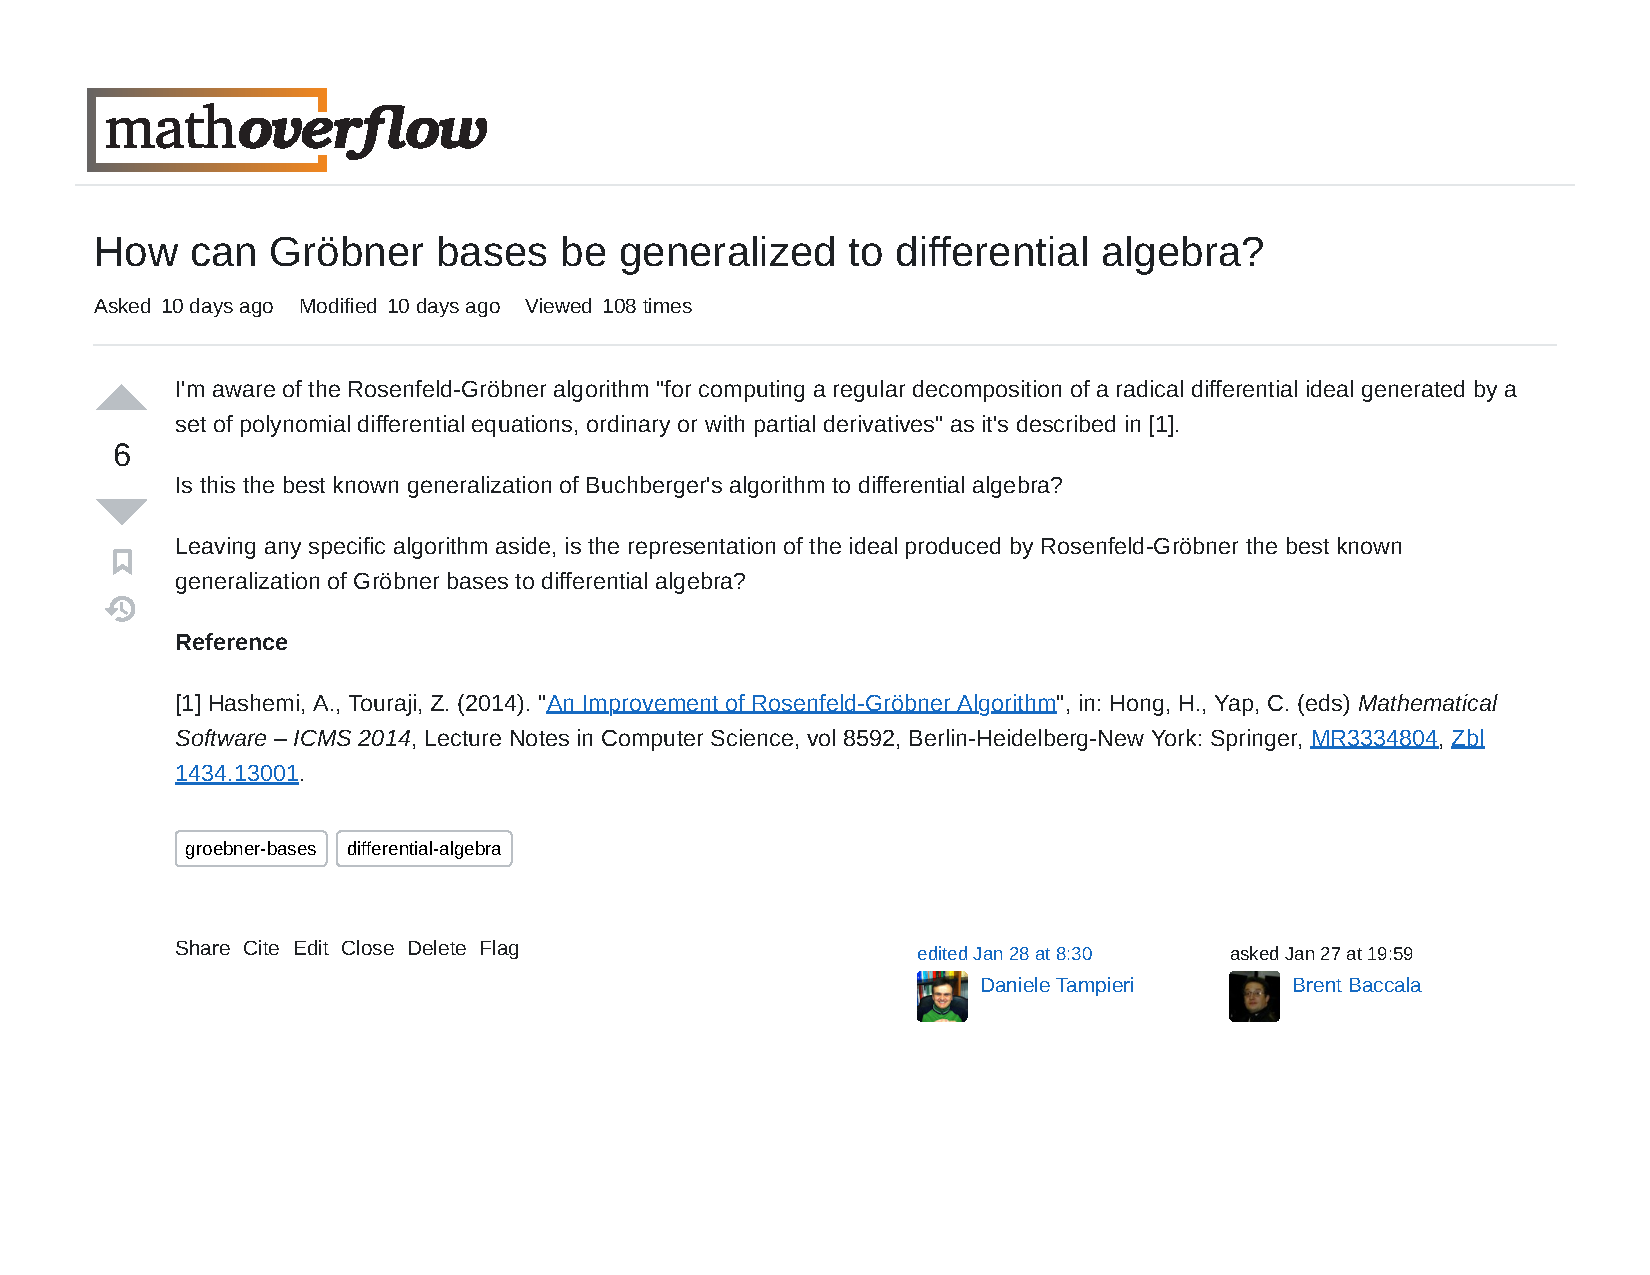
\includegraphics[width=\textwidth]{myquestion.pdf}
\end{frame}

\begin{frame}
\frametitle{The Rosenfeld-Gr\"obner Algorithm}
\begin{exampleblock}{Francois Boulier, Daniel Lazard, François Ollivier, Michel Petitot
Representation for the radical of a finitely generated differential ideal
}
\includegraphics[page=2, clip, trim=0in 0in 0in 5.2in, width=\textwidth]{blop.pdf}
\end{exampleblock}
\end{frame}

\begin{frame}[fragile]
\frametitle{Hydrogen ansatz 5}
\begin{semiverbatim}
\tiny
        # A second-order homogeneous ODE: D(B) d^2 Zeta/dB^2 - M(B) dZeta/dB - N(B) Zeta = 0
        # where D(B), M(B), and N(B) are linear polynomials in B, which is itself a linear polynomial
        #
        # Homogenization forces B and D to be non-zero; B is also forced to be non-constant

        (Bvars, B) = trial_polynomial('b', coordinates, roots, 1, constant=None)
        Psi = Zeta(B)
        (Dvars, D) = trial_polynomial('d', [B], [], 1)
        (Mvars, M) = trial_polynomial('m', [B], [], 1)
        (Nvars, N) = trial_polynomial('n', [B], [], 1)

        pre_subs = {DD[0,0](Zeta)(B) : (M * DD[0](Zeta)(B) + N * Zeta(B)) / D}

        def H(Psi):
            return - 1/2 * Del(Psi,[x1,y1,z1]) - (1/r1)*Psi

\textcolor{blue}{sage:} load('helium.sage')
\textcolor{blue}{sage:} prep_hydrogen(5)
\textcolor{blue}{sage:} multi_init()
\textcolor{blue}{sage:} multi_expand()
\textcolor{blue}{sage:} random_numerical(homogenize=1)

...
0.009979418947198756                 0.11 sec
9.395154242474284e-06                0.11 sec
6.6733587209712955e-15               0.10 sec
6.169694306802097e-32                0.12 sec


\end{semiverbatim}
\end{frame}

\begin{frame}[fragile]
\frametitle{Hydrogen ansatz 5}
\begin{semiverbatim}
\tiny

\textcolor{blue}{sage:} eq_a

-1/2*(((b2*r1*x1 + b4*r1*y1 + b6*r1*z1 + b0*r1 + b1*x1 + b3*y1 + b5*z1)*m1 + m0)*DZeta
+ ((b2*r1*x1 + b4*r1*y1 + b6*r1*z1 + b0*r1 + b1*x1 + b3*y1 + b5*z1)*n1 + n0)*Zeta)
   *(b2*r1 + b2*x1^2/r1 + b4*x1*y1/r1 + b6*x1*z1/r1 + b1 + b0*x1/r1)^2
   /((b2*r1*x1 + b4*r1*y1 + b6*r1*z1 + b0*r1 + b1*x1 + b3*y1 + b5*z1)*d1 + d0)
- 1/2*(((b2*r1*x1 + b4*r1*y1 + b6*r1*z1 + b0*r1 + b1*x1 + b3*y1 + b5*z1)*m1 + m0)*DZeta
+ ((b2*r1*x1 + b4*r1*y1 + b6*r1*z1 + b0*r1 + b1*x1 + b3*y1 + b5*z1)*n1 + n0)*Zeta)
   *(b4*r1 + b2*x1*y1/r1 + b4*y1^2/r1 + b6*y1*z1/r1 + b3 + b0*y1/r1)^2
   /((b2*r1*x1 + b4*r1*y1 + b6*r1*z1 + b0*r1 + b1*x1 + b3*y1 + b5*z1)*d1 + d0)
- 1/2*(((b2*r1*x1 + b4*r1*y1 + b6*r1*z1 + b0*r1 + b1*x1 + b3*y1 + b5*z1)*m1 + m0)*DZeta
+ ((b2*r1*x1 + b4*r1*y1 + b6*r1*z1 + b0*r1 + b1*x1 + b3*y1 + b5*z1)*n1 + n0)*Zeta)
   *(b6*r1 + b2*x1*z1/r1 + b4*y1*z1/r1 + b6*z1^2/r1 + b5 + b0*z1/r1)^2
   /((b2*r1*x1 + b4*r1*y1 + b6*r1*z1 + b0*r1 + b1*x1 + b3*y1 + b5*z1)*d1 + d0)
- E*Zeta - 1/2*DZeta*(3*b2*x1/r1 - b2*x1^3/r1^3 + b4*y1/r1 - b4*x1^2*y1/r1^3 + b6*z1/r1
- b6*x1^2*z1/r1^3 + b0/r1 - b0*x1^2/r1^3) - 1/2*DZeta*(b2*x1/r1 + 3*b4*y1/r1 - b2*x1*y1^2/r1^3
- b4*y1^3/r1^3 + b6*z1/r1 - b6*y1^2*z1/r1^3 + b0/r1 - b0*y1^2/r1^3) - 1/2*DZeta*(b2*x1/r1
+ b4*y1/r1 + 3*b6*z1/r1 - b2*x1*z1^2/r1^3 - b4*y1*z1^2/r1^3 - b6*z1^3/r1^3 + b0/r1 - b0*z1^2/r1^3) - Zeta/r1


\end{semiverbatim}
\end{frame}

\begin{frame}[fragile]
\frametitle{Hydrogen ansatz 5}
\begin{semiverbatim}
\tiny

(E, 4.6673330021180737e-20)
(b0, 1.0)
(b1, 0.464918758265008)
(b2, 4.9956745914527553e-20)
(b3, 0.5179110625786596)
(b4, -1.6316396076549894e-19)
(b5, 0.7180659297529489)
(b6, 8.416841906183793e-20)
(d0, -1.2625718788062294e-26)
(d1, 1.0)
(m0, -1.0)
(m1, 1.0711161751949155e-20)
(n0, -1.0)
(n1, -6.556316253156553e-20)

sage: roots_to_rs(B)

b2*r1*x1 + b4*r1*y1 + b6*r1*z1 + b0*r1 + b1*x1 + b3*y1 + b5*z1

sage: roots_to_rs(D)

(b2*r1*x1 + b4*r1*y1 + b6*r1*z1 + b0*r1 + b1*x1 + b3*y1 + b5*z1)*d1 + d0

sage: roots_to_rs(M)

(b2*r1*x1 + b4*r1*y1 + b6*r1*z1 + b0*r1 + b1*x1 + b3*y1 + b5*z1)*m1 + m0

sage: roots_to_rs(N)

(b2*r1*x1 + b4*r1*y1 + b6*r1*z1 + b0*r1 + b1*x1 + b3*y1 + b5*z1)*n1 + n0

\end{semiverbatim}
\vskip 0pt plus 100fill
\end{frame}

\begin{frame}[fragile]
\frametitle{Hydrogen ansatz 5}

The ODE:
\vskip 20pt
\centerline{$B = r + 0.464918758265 x + 0.5179110625786 y + 0.7180659297529 z$}
\vskip 20pt
\centerline{$B \frac{d^2\Psi}{dB^2} + \frac{d\Psi}{dB} + \Psi = 0$}
\vskip 20pt

The PDE:

\vskip 20pt

\centerline{$-\frac{1}{2} \Delta \Psi - \frac{1}{r}\Psi = 0$}
\vskip 20pt
\centerline{$-\frac{1}{2} \triangledown^2 \Psi - \frac{1}{r}\Psi = 0$}
\vskip 20pt

\centerline{$-\frac{1}{2} \left(\frac{\delta^2}{\delta^2 x} + \frac{\delta^2}{\delta^2 y} + \frac{\delta^2}{\delta^2 z}\right) \Psi - \frac{1}{r}\Psi = 0$}



\end{frame}

\begin{frame}[fragile]
%%\frametitle{Hydrogen ansatz 5}
\scriptsize

\hbox{Claim: this ODE}\centerline{$B \frac{d^2\Psi}{dB^2} + \frac{d\Psi}{dB} + \Psi = 0 \qquad\qquad B = r + x$}
\vskip 20pt

\hbox{Satisfies this PDE}\centerline{$\frac{1}{2} \left(\frac{\delta^2}{\delta^2 x} + \frac{\delta^2}{\delta^2 y} + \frac{\delta^2}{\delta^2 z}\right) \Psi + \frac{1}{r}\Psi = 0$}

\vskip 20pt

\centerline{$\frac{\delta}{\delta x} \Psi = \frac{d B}{d x} \frac{d}{d B}  \Psi = \left(\frac{x}{r} + 1\right)\Psi' \qquad \frac{\delta}{\delta y} \Psi = \frac{d B}{d y} \frac{d}{d B}  \Psi = \frac{y}{r} \Psi' \qquad \frac{\delta}{\delta z} \Psi = \frac{d B}{d z} \frac{d}{d B}  \Psi = \frac{z}{r} \Psi' $}

\vskip 20pt

\centerline{$\frac{\delta^2}{\delta^2 x} \Psi = \frac{\delta}{\delta x} \left(\left(\frac{x + r}{r}\right) \Psi'\right) = \left(\frac{r(1 + \frac{x}{r}) - \frac{x}{r}(r+x)}{r^2} \Psi' + \left(\frac{x}{r} + 1\right)\frac{dB}{dx}\frac{d}{dB}\Psi'\right)$}
\centerline{$= \left(\frac{r(r + x) - x(r+x)}{r^3} \Psi' + \left(\frac{x}{r} + 1\right)^2\Psi''\right) = \left(\frac{r^2 - x^2}{r^3} \Psi' + \left(\frac{x}{r} + 1\right)^2\Psi''\right)$}

\vskip 20pt

\centerline{$\frac{\delta^2}{\delta^2 y} \Psi = \frac{\delta}{\delta y} \left(\left(\frac{y}{r}\right) \Psi'\right) = \left(\frac{r - \frac{y}{r}(y)}{r^2} \Psi' + \left(\frac{y}{r}\right)^2\Psi''\right) = \left(\frac{r^2 - y^2}{r^3} \Psi' + \left(\frac{y}{r}\right)^2\Psi''\right)$}

\vskip 20pt

\centerline{$\left(\frac{\delta^2}{\delta^2 x} + \frac{\delta^2}{\delta^2 y} + \frac{\delta^2}{\delta^2 z}\right) \Psi = \left(\frac{2}{r}\Psi' + \left(\frac{x^2}{r^2} + 2\frac{x}{r} + 1 + \frac{y^2}{r^2} + \frac{z^2}{r^2}\right)\Psi''\right)  = \left(\frac{2}{r}\Psi' + \left(2 + 2\frac{x}{r}\right)\Psi''\right)$}

\vskip 20pt
\centerline{$\left(\frac{1}{r}\Psi' + \left(1 + \frac{x}{r}\right)\Psi''\right) + \frac{1}{r}\Psi = 0 \qquad\Rightarrow\qquad \Psi' + \left(r + x\right)\Psi'' + \Psi = 0$}

\end{frame}

\begin{frame}[fragile]
\frametitle{Hydrogen ansatz 5}
\small

\centerline{$B \frac{d^2\Psi}{dB^2} + \frac{d\Psi}{dB} + \Psi = 0$}
\vskip 10pt
\centerline{Is the solution liovillian?}
\centerline{Kovacic says no!}

\includegraphics[page=3,clip,trim=0in 7.2in 0in 1.2in, width=\textwidth]{Kovacic.pdf}

\centerline{$\frac{d^2\Psi}{dB^2} + \frac{1}{B}\frac{d\Psi}{dB} + \frac{1}{B}\Psi = 0$}

$$z=e^{\frac{1}{2}\int\frac{1}{x}} y = e^{\frac{1}{2}\ln x} y = \sqrt{x}y$$

$$z'' + \left(\frac{1}{x} + \frac{1}{4x^2}\right) z = 0$$

\end{frame}

\begin{frame}[fragile]
\frametitle{Hydrogen ansatz 5}
\small

$$z'' + \left(\frac{1}{x} + \frac{1}{4x^2}\right) z = z'' + \left(\frac{4x + 1}{4x^2}\right) z = 0$$

\includegraphics[page=6,clip,trim=0in 2in 0in 5in, width=\textwidth]{Kovacic.pdf}

{\tiny Source: Jerald J. Kovacic, {\it An Algorithm for Solving Second Order Linear Homogeneous Differential Equations}}
\end{frame}

\begin{frame}[fragile]
\frametitle{Hydrogen ansatz 5}
\small

$$z'' + \left(\frac{1}{x} + \frac{1}{4x^2}\right) z = z'' + \left(\frac{4x + 1}{4x^2}\right) z = 0$$

\includegraphics[page=16,clip,trim=0in 4in 0in 3.6in, width=\textwidth]{Kovacic.pdf}

$$E_0 = \{2, 2\pm2\sqrt{2}\}\qquad E_\infty = \{ 1\} $$

\end{frame}

\begin{frame}[fragile]
\frametitle{Hydrogen ansatz 5}
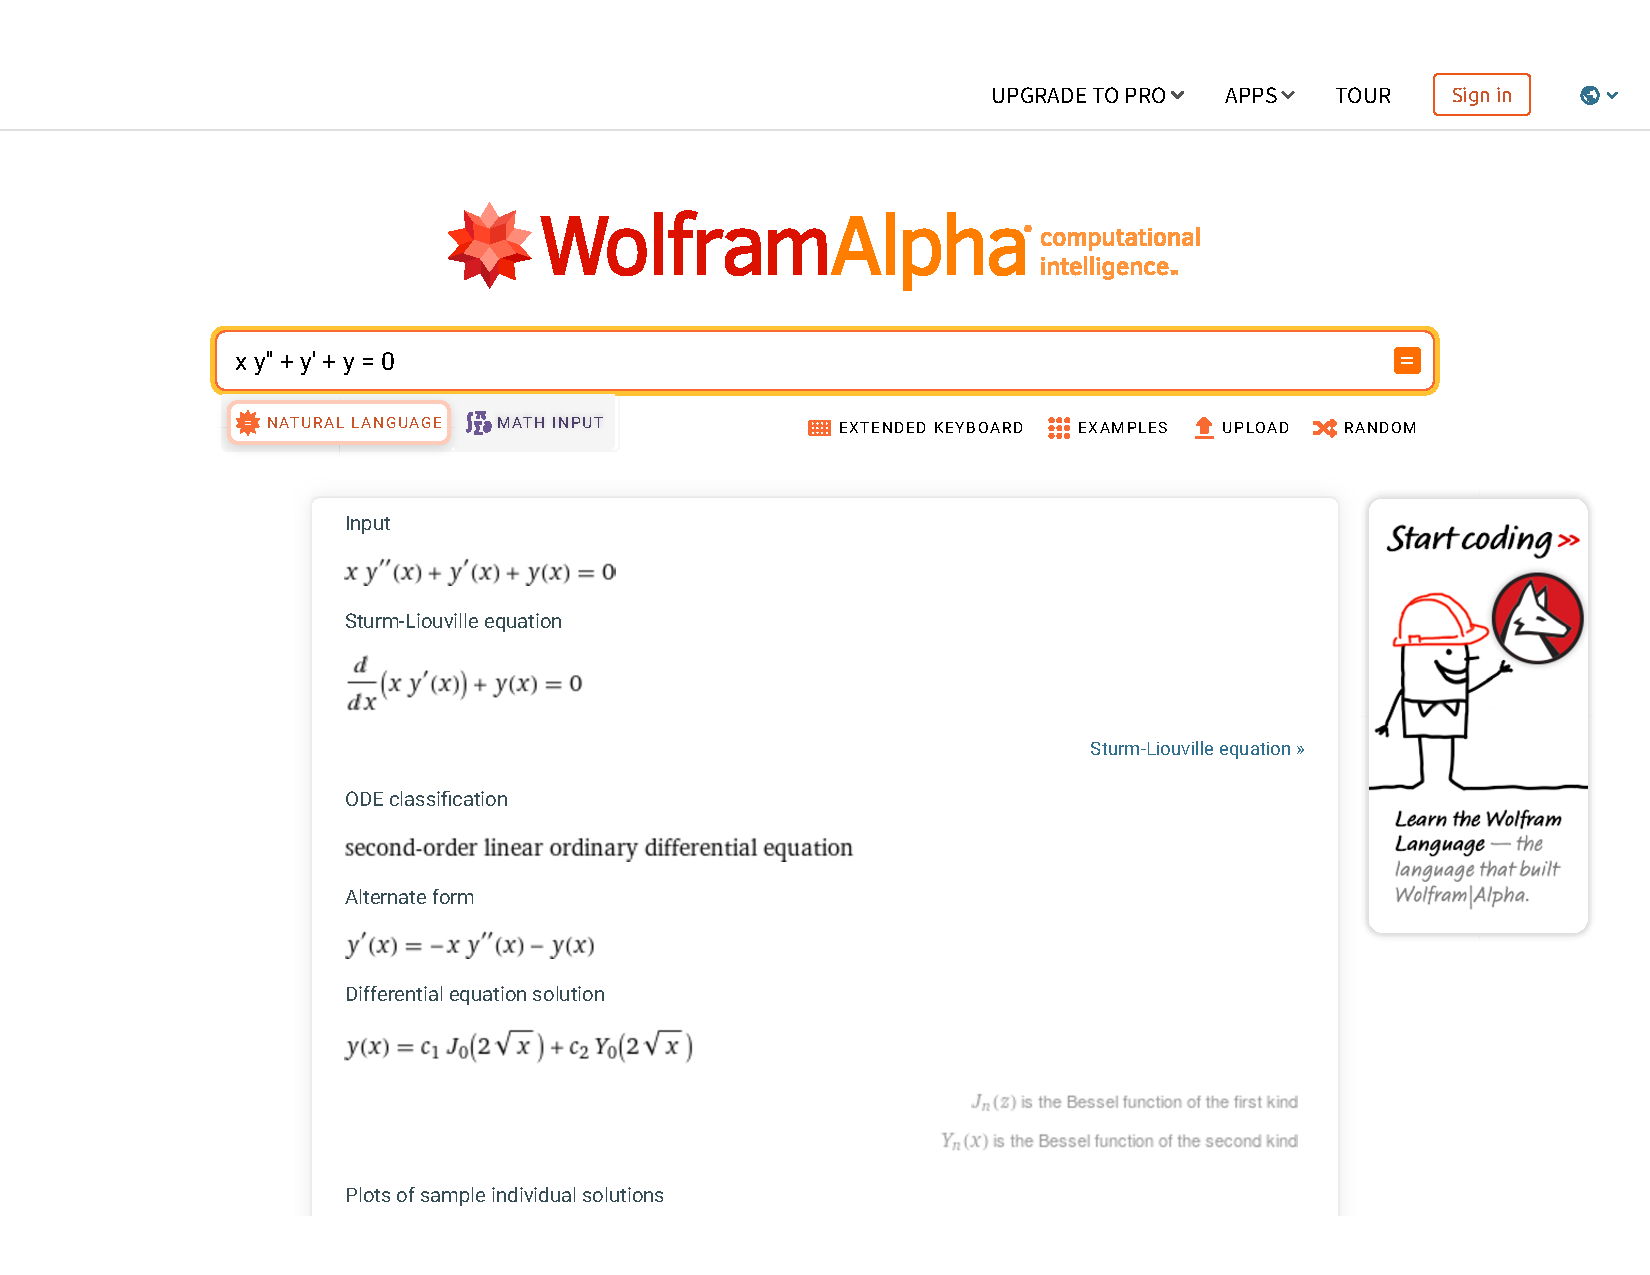
\includegraphics[page=1, clip, trim=0in 0in 0in 1in, width=\textwidth]{Wolfram Alpha.pdf}
\end{frame}

\begin{frame}[fragile]
\frametitle{Bessel functions}
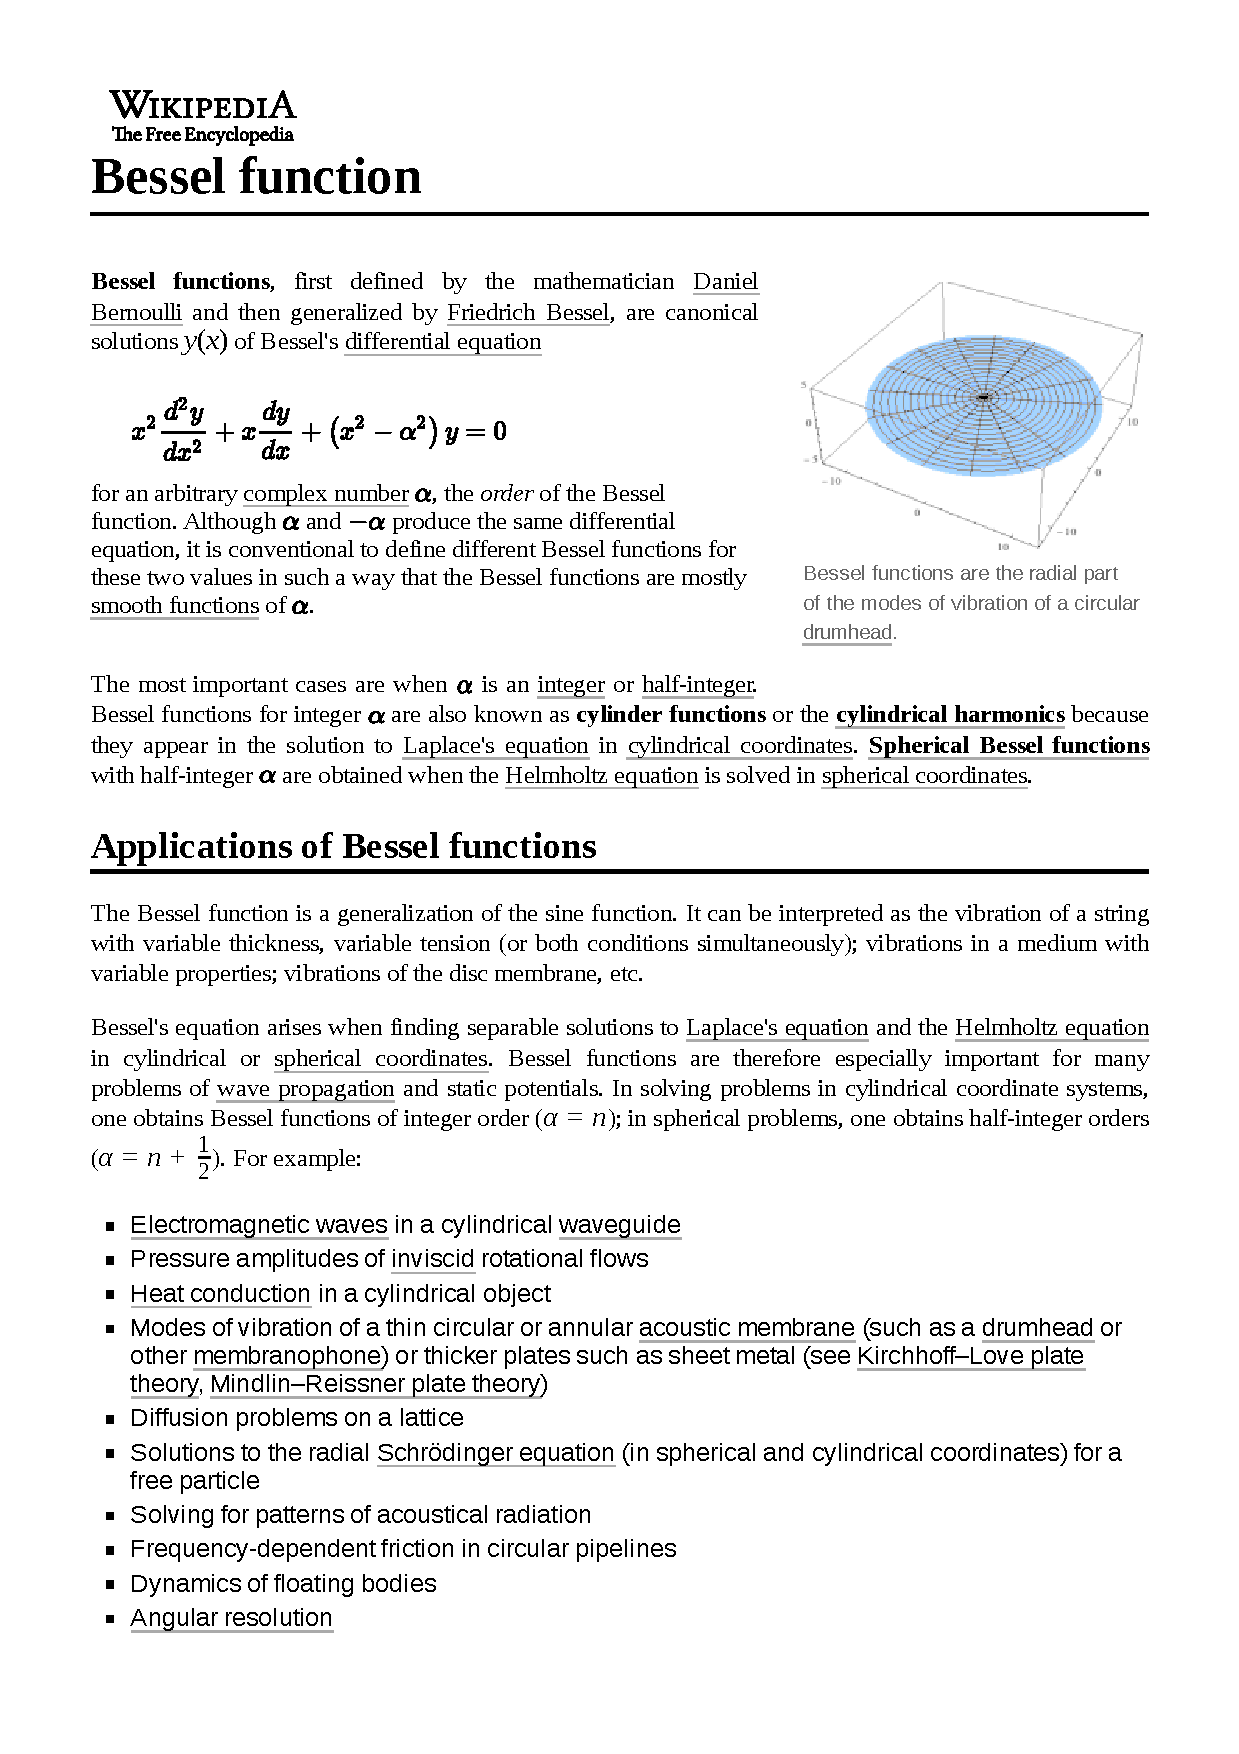
\includegraphics[page=1, clip, trim=0in 0in 0in 0in, width=\textwidth]{Bessel function.pdf}
\end{frame}

\begin{frame}
\begin{center}
%Bessel functions solve $x^2 y'' + x y' + (x^2 - \alpha^2)y = 0$.
%\vskip 20pt

$J_0$ and $Y_0$ ($\alpha = 0$) solve $x^2 y'' + x y' + x^2 y = 0$.

\vskip 20pt
Claim: $z(x) = J_0(2\sqrt{x})$ solves $x z'' + z' + z = 0$

\vskip 20pt
So, does $z(x) = (y\circ f)(x)$ and $f(x) = 2\sqrt{x}$ solve $x z'' + z' + z = 0$?

\vskip 20pt 

$z' = \frac{dz}{dx} = y'(2\sqrt{x}) \cdot \frac{1}{\sqrt{x}}$

$z'' = y''(2\sqrt{x}) \cdot \frac{1}{\sqrt{x}} \cdot \frac{1}{\sqrt{x}} + y'(2\sqrt{x}) \left(-\frac{1}{2x^{3/2}}\right)$

\vskip 20pt 

$4 x^2 z'' = 4 x y''(2\sqrt{x}) - 2 \sqrt{x} y'(2\sqrt{x})$

$ = \left[ -2 \sqrt{x} y'(2\sqrt{x}) - 4x y(2\sqrt{x})\right] - 2 \sqrt{x} y'(2\sqrt{x})$

$ = -4 \sqrt{x} y'(2\sqrt{x}) - 4x y(2\sqrt{x})$
$ = -4 x z'(x) - 4x z(x)$

\vskip 20pt
$4 x^2 z'' = -4 x z'(x) - 4x z(x)$

$x z'' = - z'(x) - z(x)$
\end{center}
\end{frame}

\begin{frame}
\begin{exampleblock}{}
\begin{center}
\vskip 20pt
\Huge
Part 3: Optimization
\vskip 6pt
\ 
\end{center}
\end{exampleblock}
\end{frame}

\begin{frame}[fragile]
\frametitle{numpy code to construct monomials \break (graded lexicographic order)}
\begin{semiverbatim}
\tiny
    # Now we want to evaluate possibly millions of polynomials, as
    # well as their first derivatives.  Using Sage symbolic
    # expressions is slow and consumes much memory, so we use scipy
    # sparse matrices instead.  Each row in the matrix is a polynomial
    # and each column corresponds to a monomial.  The matrix entry is
    # that monomial's coefficient.  We can then evaluate all the
    # polynomials at once by forming a vector of all the monomials (up
    # to a given maximum degree) and multiplying it by the matrix.

    # Given a vector, generate a multi-vector of the vector itself,
    # then all the biproducts of the vector elements, then all the
    # triproducts of the vector elements, etc.
    #
    # [a,b,c]
    # [a,b,c] * a, [b,c] * b, [c] * c = [a^2, a*b, a*c, b^2, b*c, c^2]
    #
    # Now we stack them all together, and get our monomials in graded lexicographic order
    #
    #   -> [1,a,b,c,a^2,a*b,a*c,b^2,b*c,c^2,a^3,a^2*b,a^2*c,a*b^2,a*b*c,a*c^2,a*b^2,b^2*c,b*c^2,c^3]

    def generate_multi_vector(self, v):
        npv = np.array(v)
        stack = [[1], npv]
        for d in range(1, self.max_degree):
            stack.append([np.hstack(stack[-1][i:]) * npv[i] for i in range(len(v))])
        res = np.hstack(tuple(flatten(stack)))
        return res

\end{semiverbatim}
\vskip 0pt plus 100fill
\end{frame}

\begin{frame}[fragile]
\frametitle{numpy code to construct monomials \break (graded lexicographic order)}

Same idea, but for first derivatives

\begin{semiverbatim}
\tiny
    def generate_multi_D_vector(self, v, var):
        ind = coeff_vars.index(var)

        npv = np.array(v)

        firsts = np.zeros(npv.size)
        firsts[ind] = int(1)
        D_stack = [[0], firsts]
        stack = [[1], npv]

        for d in range(1, self.max_degree):
            D_stack.append([np.hstack(stack[-1][i:]) * firsts[i] + np.hstack(D_stack[-1][i:]) * npv[i]
                            for i in range(len(v))])
            stack.append([np.hstack(stack[-1][i:]) * npv[i] for i in range(len(v))])

        res = np.hstack(tuple(flatten(D_stack)))

        return res
\end{semiverbatim}
\vskip 0pt plus 100fill
\end{frame}

\begin{frame}[fragile]
\frametitle{numpy code to evaluate a system polynomials}

The coefficients of our polynomials have already been assembled into a (sparse) matrix.

Once we've constructed the monomial vector, evaluating them is easy.

\begin{semiverbatim}
\tiny
    @async_result
    def eval_fns(self, vec):
        r"""
        Evaluate our polynomials

        INPUT:

        - ``vec`` -- a vector of real values for all coeff_vars

        OUTPUT:

        - a vector of all of our polynomials, evaluated at ``vec``
        """
        multivec = self.generate_multi_vector(vec)
        return self.dot(multivec)

\end{semiverbatim}
\vskip 0pt plus 100fill
\end{frame}

\begin{frame}[fragile]
\frametitle{scipy sparse matrices}
\includegraphics[width=\textwidth]{scipy_sparse.png}
\end{frame}

\begin{frame}[fragile]
\frametitle{scipy's sparse CSR matrix vector multiplication routine}
%% ~/src/scipy/scipy/sparse/sparsetools/csr.h
\begin{semiverbatim}
\tiny
/* Compute Y += A*X for CSR matrix A and dense vectors X,Y
 *
 * Input Arguments:
 *   I  n_row         - number of rows in A
 *   I  n_col         - number of columns in A
 *   I  Ap[n_row+1]   - row pointer
 *   I  Aj[nnz(A)]    - column indices
 *   T  Ax[nnz(A)]    - nonzeros
 *   T  Xx[n_col]     - input vector
 *
 * Output Arguments:
 *   T  Yx[n_row]     - output vector
 *
 * Note:
 *   Output array Yx must be preallocated
 *
 *   Complexity: Linear.  Specifically O(nnz(A) + n_row)
 */
template <class I, class T>
void csr_matvec(const I n_row, const I n_col, const I Ap[],
                const I Aj[],  const T Ax[],  const T Xx[], T Yx[])
\{
    for(I i = 0; i < n_row; i++)\{
        T sum = Yx[i];
        for(I jj = Ap[i]; jj < Ap[i+1]; jj++)\{
            sum += Ax[jj] * Xx[Aj[jj]];
        \}
        Yx[i] = sum;
    \}
\}

\end{semiverbatim}
\vskip 0pt plus 100fill
\end{frame}

\begin{frame}[fragile]
\frametitle{gcc's assembly code for the inner loop ({\tt -mavx2 -O3})}
%% cat sparse1.c
%% objdump -dwr --no-show-raw-insn sparse1.o | sed 's/#[^<]*<[^>]*>//' | grep '^ *[0-9a-f]*:' | column -t
\begin{semiverbatim}
\tiny
double sum;

const int Aj[4];
const double Ax[4];
const double Xx[4];

void vecmult(void)
\{
    for(int jj = 0; jj < 4; jj++) \{
        sum += Ax[jj] * Xx[Aj[jj]];
    \}
\}

0:   endbr64
4:   movslq       0x0(%rip),%rdx             7:   R_X86_64_PC32  Aj-0x4
b:   lea          0x0(%rip),%rax             e:   R_X86_64_PC32  Xx-0x4
12:  vmovsd       0x0(%rip),%xmm1            16:  R_X86_64_PC32  sum-0x4
1a:  vmovsd       0x0(%rip),%xmm2            1e:  R_X86_64_PC32  Ax+0x4
22:  vmovsd       0x0(%rip),%xmm3            26:  R_X86_64_PC32  Ax+0xc
2a:  vmovsd       0x0(%rip),%xmm4            2e:  R_X86_64_PC32  Ax+0x14
32:  vmovsd       (%rax,%rdx,8),%xmm0
37:  movslq       0x0(%rip),%rdx             3a:  R_X86_64_PC32  Aj
3e:  vfmadd132sd  0x0(%rip),%xmm1,%xmm0      43:  R_X86_64_PC32  Ax-0x4
47:  vfmadd231sd  (%rax,%rdx,8),%xmm2,%xmm0
4d:  movslq       0x0(%rip),%rdx             50:  R_X86_64_PC32  Aj+0x4
54:  vfmadd231sd  (%rax,%rdx,8),%xmm3,%xmm0
5a:  movslq       0x0(%rip),%rdx             5d:  R_X86_64_PC32  Aj+0x8
61:  vfmadd231sd  (%rax,%rdx,8),%xmm4,%xmm0
67:  vmovsd       %xmm0,0x0(%rip)            6b:  R_X86_64_PC32  sum-0x4
6f:  retq

\end{semiverbatim}
\vskip 0pt plus 100fill
\end{frame}

\begin{frame}[fragile]
\frametitle{Intel VFMADD132SD instruction}
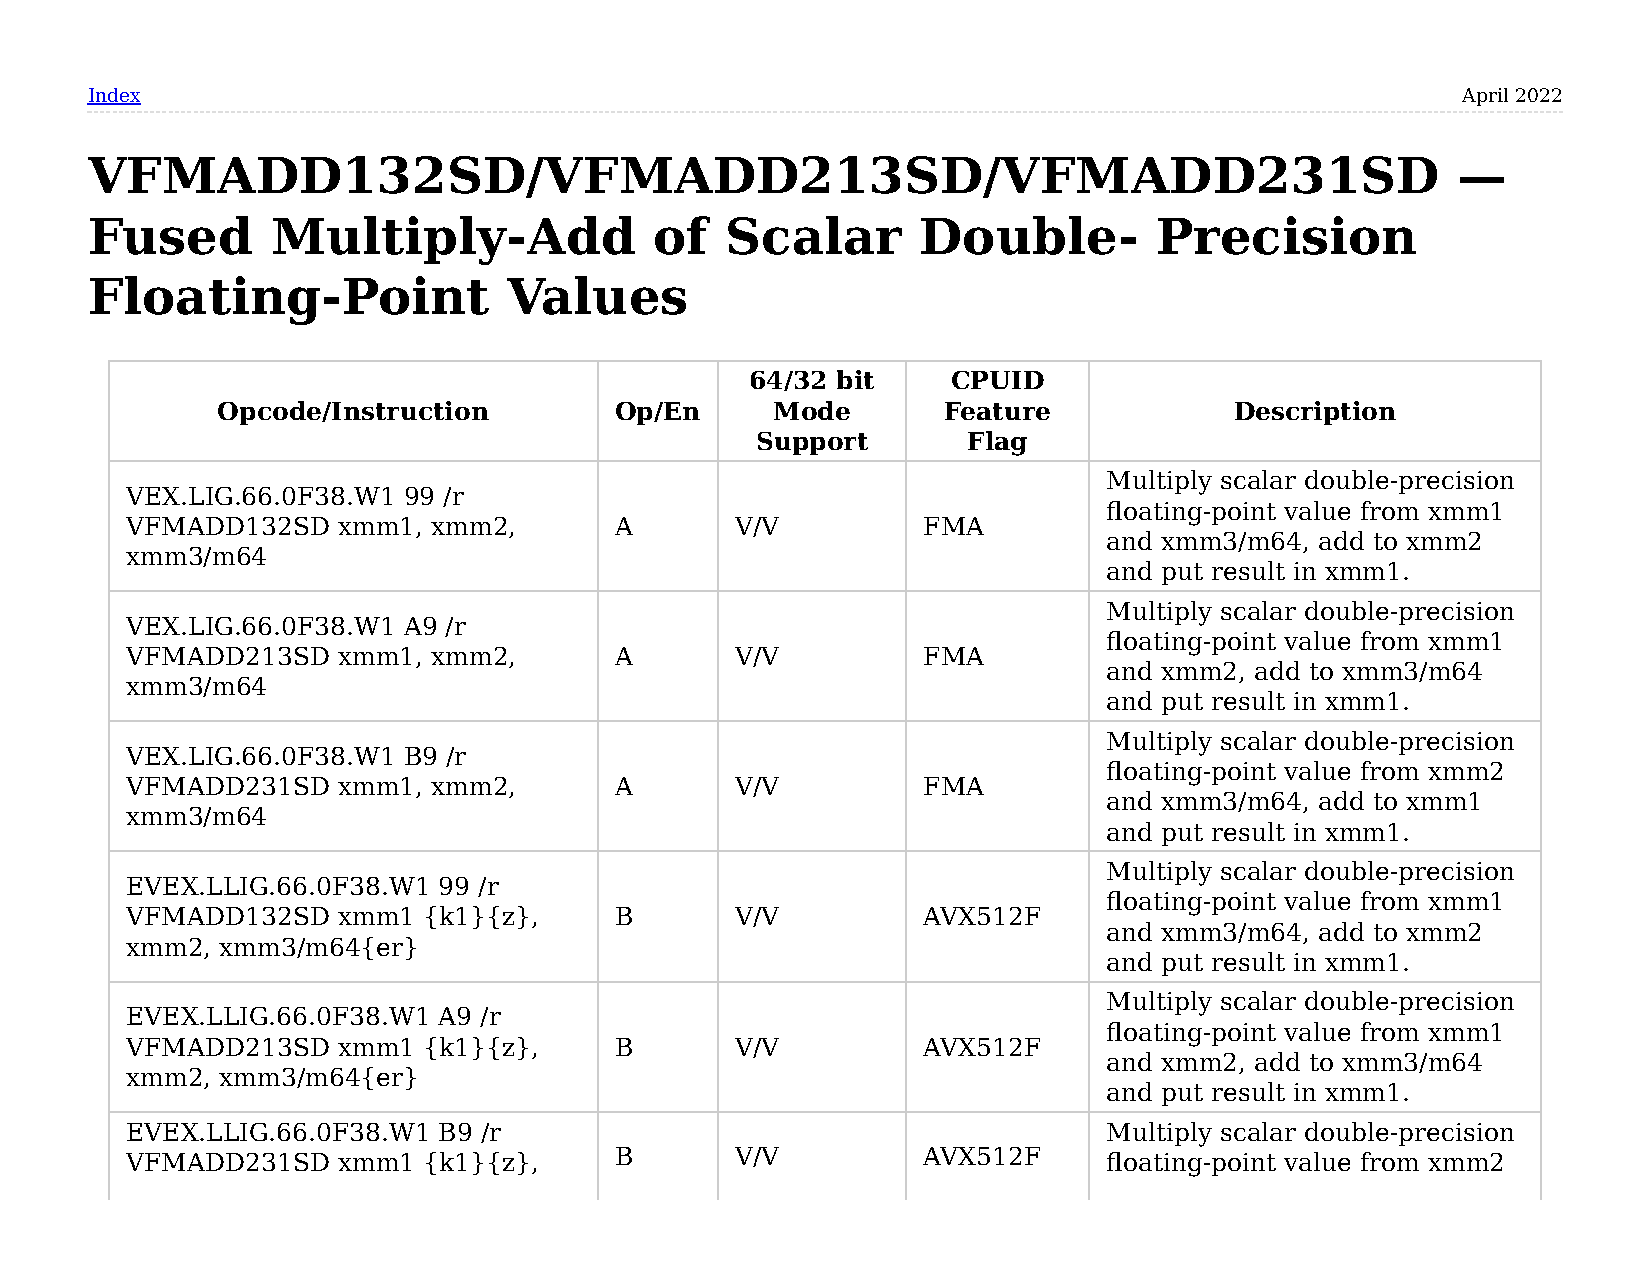
\includegraphics[page=1, clip, trim=0in 2.9in 0in 0.75in, width=\textwidth]{FVMADD132SD.pdf}

\includegraphics[page=4, clip, trim=0in 3.75in 0in 3.5in, width=\textwidth]{FVMADD132SD.pdf}
\end{frame}

\begin{frame}[fragile]
\frametitle{Improvement: using an array of accumulators}
%% cat sparse4.c
%% objdump -dwr --no-show-raw-insn sparse4.o | sed 's/#[^<]*<[^>]*>//' | grep '^ *[0-9a-f]*:' | column -t
\begin{semiverbatim}
\scriptsize

double tmp1[4] __attribute__((aligned(32)));
double tmp2[4] __attribute__((aligned(32)));
double tmp3[4] __attribute__((aligned(32)));

void vecmult(void)
\{
    for (int i=0; i<4; i++) \{
        tmp3[i] += tmp1[i] * tmp2[i];
    \}
\}

0:   endbr64
4:   vmovapd     0x0(%rip),%ymm1        8:   R_X86_64_PC32  tmp1-0x4
c:   vmulpd      0x0(%rip),%ymm1,%ymm0  10:  R_X86_64_PC32  tmp2-0x4
14:  vaddpd      0x0(%rip),%ymm0,%ymm0  18:  R_X86_64_PC32  tmp3-0x4
1c:  vmovapd     %ymm0,0x0(%rip)        20:  R_X86_64_PC32  tmp3-0x4
24:  vzeroupper
27:  retq

\end{semiverbatim}
\vskip 0pt plus 100fill
\end{frame}

\begin{frame}[fragile]
\frametitle{Intel MULPD instruction}
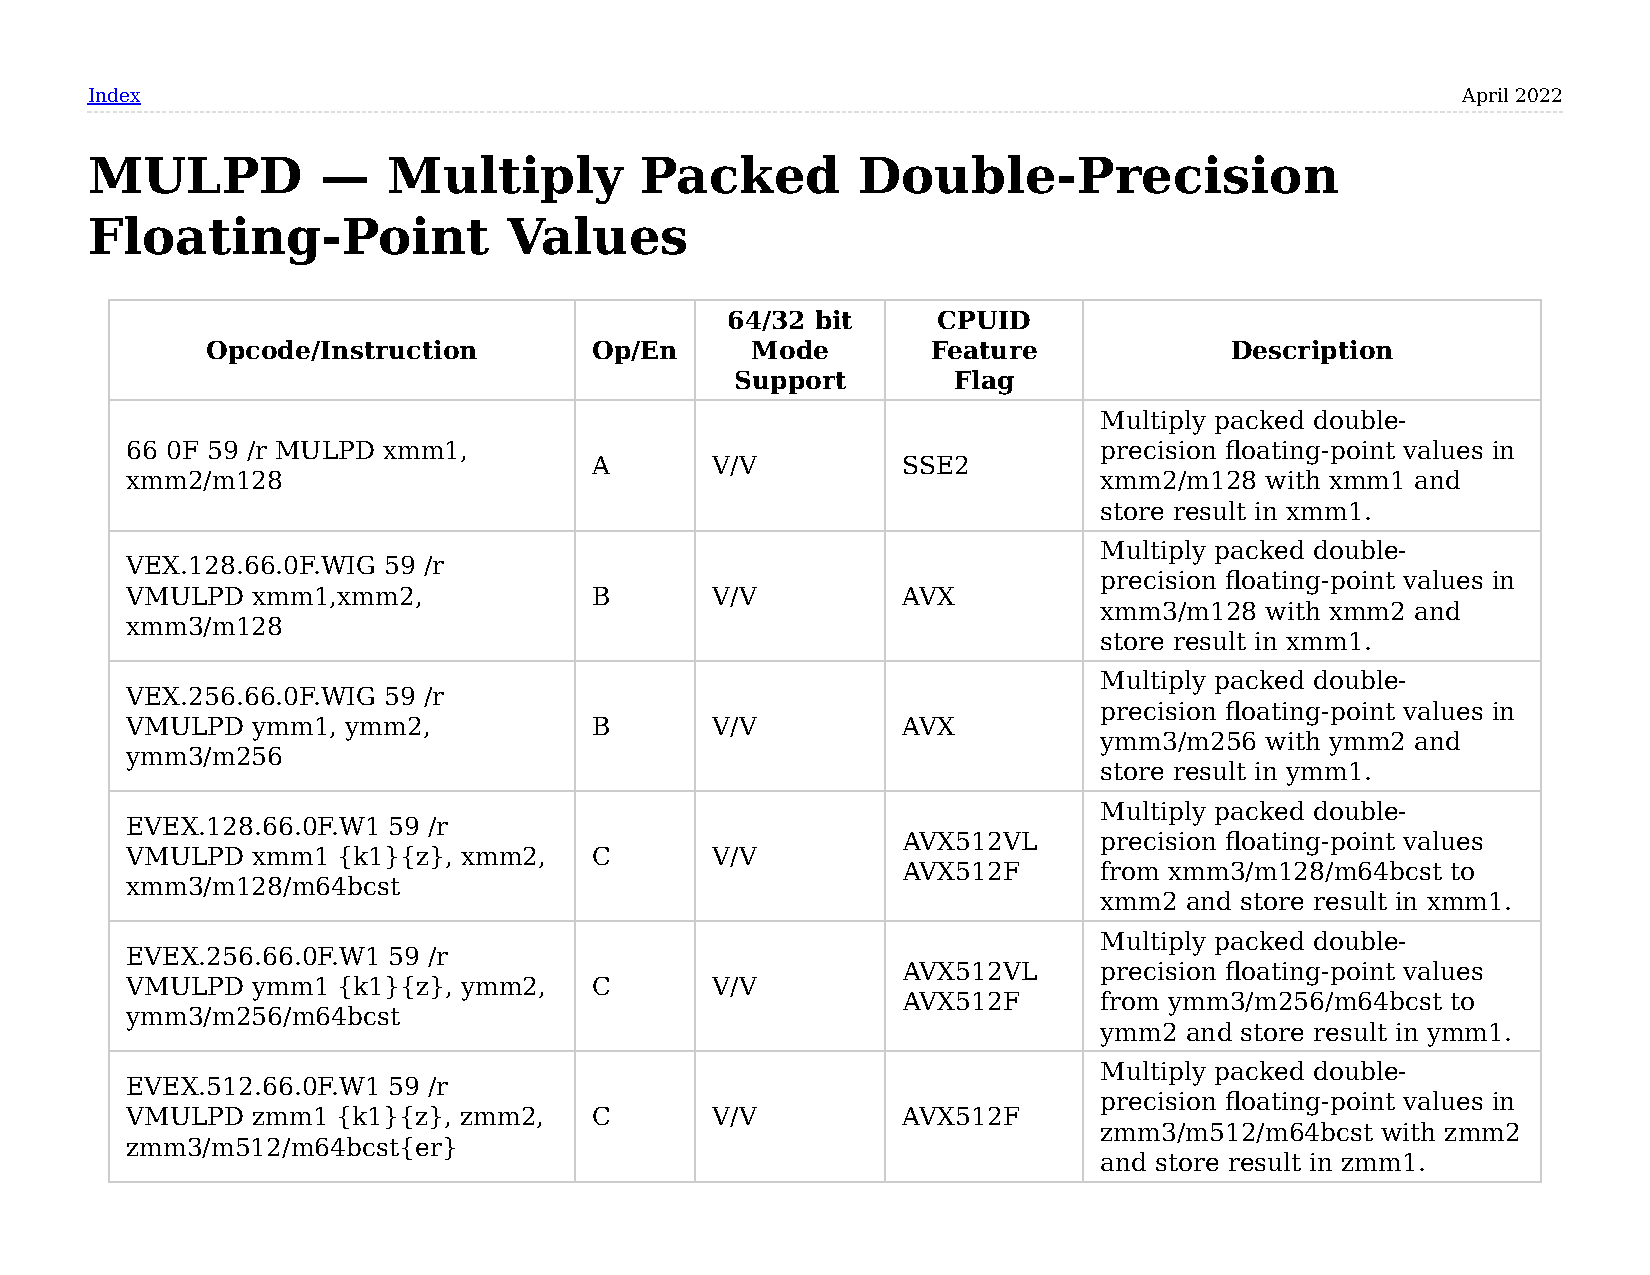
\includegraphics[page=1, clip, trim=0in 3.2in 0in 0.75in, width=\textwidth]{mulpd.pdf}

\includegraphics[page=2, clip, trim=0in 5in 0in 2.2in, width=\textwidth]{mulpd.pdf}

\includegraphics[page=3, clip, trim=0in 2.6in 0in 4.2in, width=\textwidth]{mulpd.pdf}
\end{frame}

\end{document}
